\documentclass[11pt,letterpaper,twoside]{book}

% ==========================================
% SIRCAS Reference Manual
% Sound processor, memory map, voices, filter and sequencer
% ==========================================

% Manual-specific strings used by the shared preamble (footer, PDF metadata).
\newcommand{\sircManualFooter}{SIRCAS REFERENCE MANUAL}
\newcommand{\sircManualTitle}{SIRCAS Reference Manual}
\newcommand{\sircManualSubject}{SIRCAS, the SIRC Audio System: sound processor, memory map, voices, filter and sequencer}

% Names of this manual and its sibling, for references within the set.
\newcommand{\audiomanual}{\textit{SIRCAS Reference Manual}}
\newcommand{\videomanual}{\textit{SIRCADA Reference Manual}}

% ==========================================
% Shared preamble for the SIRC-1 manuals (docs/reference and docs/hardware)
% ==========================================

% ------------------------------------------------------------
% Encoding and typography
% ------------------------------------------------------------

\usepackage[utf8]{inputenc}
\usepackage[T1]{fontenc}

% Helvetica-compatible sans serif.
% TeX Gyre Heros is a high-quality Helvetica replacement.
\usepackage{tgheros}
\renewcommand{\familydefault}{\sfdefault}

% Courier-compatible monospace.
\usepackage{tgcursor}

% Better character spacing / kerning.
\usepackage{microtype}

% ------------------------------------------------------------
% Page layout
% ------------------------------------------------------------

\usepackage{geometry}

\geometry{
	a4paper,
	left=25mm,
	right=20mm,
	top=22mm,
	bottom=25mm,
	headheight=14pt
}

% The book class flushes page bottoms in two-sided mode. With many [H] tables
% that cuts pages short, so the leftover space gets spread through lists and
% paragraphs instead. Let short pages stay short.
\raggedbottom

% ------------------------------------------------------------
% General packages
% ------------------------------------------------------------

\usepackage{graphicx}
\usepackage{eso-pic}
\usepackage{xcolor}
\usepackage{fancyhdr}
\usepackage{titlesec}
\usepackage{enumitem}
\usepackage{float}

% A captioned, non-floating environment for worked assembly examples, so
% they get a real "List of Examples" (like the existing List of
% Figures/Tables) instead of a hand-maintained one. Numbered N-M (chapter
% number, then sequential within that chapter/appendix) to match the
% manual's existing "Example 13-1" convention; [H] means it never actually
% floats away from where the author placed it.
\newfloat{example}{H}{loe}[chapter]
\floatname{example}{Example}
\renewcommand{\theexample}{\thechapter-\arabic{example}}

\usepackage{tabularx}
\usepackage{booktabs}
\usepackage{multirow}
\usepackage{longtable}
\usepackage{xltabular}

\usepackage{amsmath}
\usepackage{amssymb}

\usepackage{listings}
\usepackage{bytefield}
\bytefieldsetup{endianness=big}

\usepackage{tikz}
\usepackage{tikz-timing}
\usetikzlibrary{
	shapes.geometric,
	arrows.meta,
	positioning,
	fit,
	calc
}

\usepackage{tcolorbox}
\tcbuselibrary{breakable, skins}

% Load hyperref relatively late.
\usepackage{hyperref}

% ------------------------------------------------------------
% Timing diagrams
% ------------------------------------------------------------

\tikzset{
	sirc timing diagram/.style={
			timing/slope=0,
			timing/dslope=0.15,
			timing/xunit=3.4em,
			timing/rowdist=2.2,
			timing/coldist=2.2,
		},
}

% ------------------------------------------------------------
% Colours
% ------------------------------------------------------------

\definecolor{sircred}{RGB}{255,0,0}
\definecolor{sircgray}{RGB}{110,110,110}
\definecolor{sirclightgray}{RGB}{232,232,232}
\definecolor{codebg}{RGB}{245,245,245}
\definecolor{opcodecolor}{RGB}{153,0,0}

% ------------------------------------------------------------
% Manual-specific strings
% ------------------------------------------------------------
% A manual's main.tex defines these (with \newcommand) before it inputs this
% preamble. The defaults are for the Architecture Reference Manual.

\providecommand{\sircManualFooter}{SIRC-1 ARCHITECTURE REFERENCE MANUAL}
\providecommand{\sircManualTitle}{SIRC-1 Architecture Reference Manual}
\providecommand{\sircManualSubject}{SIRCIS Instruction Set Architecture}

% Names of the manuals in the set, for references between them
\providecommand{\archmanual}{\textit{SIRC-1 Architecture Reference Manual}}
\providecommand{\hwmanual}{\textit{SIRC-1 Hardware Reference Manual}}
\providecommand{\asmmanual}{\textit{SIRC-1 Assembly Programmer's Manual}}

% ------------------------------------------------------------
% Header / footer
% ------------------------------------------------------------

\pagestyle{fancy}
\fancyhf{}

\fancyhead[LE]{\small\nouppercase{\leftmark}}
\fancyhead[RO]{\small\nouppercase{\rightmark}}
\fancyhead[RE,LO]{\small\textcolor{sircred}{DRAFT --- Not for Distribution}}

\fancyfoot[LE,RO]{\thepage}
\fancyfoot[C]{\small\textcolor{sircgray}{\sircManualFooter}}

\renewcommand{\headrulewidth}{0.8pt}
\renewcommand{\footrulewidth}{0.4pt}

% ------------------------------------------------------------
% PDF / hyperlink setup
% ------------------------------------------------------------

\hypersetup{
	colorlinks=true,
	linkcolor=sircred,
	filecolor=sircred,
	urlcolor=sircred,
	citecolor=sircred,
	bookmarksnumbered=true,
	pdfauthor={SIRC Development Team},
	pdftitle={\sircManualTitle},
	pdfsubject={\sircManualSubject},
}

% ------------------------------------------------------------
% Assembly code listings
% ------------------------------------------------------------

\lstdefinelanguage{SIRC}{
	morekeywords={
			ADDI,ADDR,ADCI,ADCR,SUBI,SUBR,SBCI,SBCR,
			ANDI,ANDR,ORRI,ORRR,XORI,XORR,
			LOAD,MOVI,MOVR,STOR,CMNI,CMNR,CNCI,CNCR,CMPI,CMPR,CPCI,CPCR,TSAI,TSAR,TSOI,TSOR,TSXI,TSXR,
			LDEA,LDEL,BRAN,LJMP,LJSR,BRSR,RETS,NOOP,
			WAIT,RETE,COPI,COPR,SHFT,EXCP,RSET,
			ETFR,ETTR,DMAR,DMAW,DMAT,MULU,MULS,DIVU,DIVS
		},
	keywordstyle=\color{sircred}\bfseries,
	sensitive=false,
	morecomment=[l]{;},
	commentstyle=\itshape\color{sircgray},
	morestring=[b]",
	stringstyle=\color{opcodecolor},
	basicstyle=\ttfamily\small,
	breaklines=true,
	showstringspaces=false
}

\lstset{
	language=SIRC,
	backgroundcolor=\color{codebg},
	frame=single,
	rulecolor=\color{sircgray},
	framesep=5pt,
	numbers=left,
	numberstyle=\tiny\color{sircgray},
	numbersep=7pt,
	xleftmargin=15pt,
	framexleftmargin=15pt,
	columns=fullflexible
}

% ------------------------------------------------------------
% Instruction reference pages
% ------------------------------------------------------------

% Modelled on the instruction-description pages of period CPU manuals (e.g.
% the M68000 Family Programmer's Reference Manual): each instruction gets a
% dedicated page (or run of pages) with the mnemonic set prominently at the
% top for flip-through lookup, rather than a boxed callout sitting in the
% middle of running text. \clearpage at the start of every entry guarantees
% two entries never share a page -- if one entry runs long, the next simply
% starts on the page after it ends. The chapter running header (already set
% by fancyhdr) carries the instruction category, matching how the M68000
% manual shows its category ("Integer Instructions", etc.) in the header of
% every instruction page.
%
% Every entry also gets its own table-of-contents/PDF-bookmark line, keyed
% off its own mnemonic and name, regardless of whether it sits directly
% under a \section of its own or is one of several instructions grouped
% under a shared \section (e.g. the Exception Unit meta-instructions in
% Chapter 16) -- so every instruction is individually findable via the ToC
% or bookmarks either way, matching the "flip through to find it" goal.
\newenvironment{instructionbox}[2]{%
	\clearpage
	\phantomsection
	\addcontentsline{toc}{section}{#1 -- #2}
	\noindent{\Huge\bfseries\color{sircred}#1}\par
	\vspace{3pt}
	\noindent{\Large\bfseries #2}\par
	\vspace{6pt}
	\titlerule
	\vspace{10pt}
}{%
}

% A compact boxed reference for one addressing mode: GENERATION, ASSEMBLER
% SYNTAX, FIELD ENCODING, and INSTRUCTION WORD COUNT, matching the M68000
% PRM's per-mode encoding box. Unlike instructionbox, this does not force a
% page break -- there are only seven addressing modes and each is short
% enough that several fit per page.
\newtcolorbox{addrmodebox}[1]{
	colback=sirclightgray,
	colframe=sircred,
	coltitle=black,
	fonttitle=\bfseries\large,
	title=#1,
	arc=0mm,
	boxrule=0.8pt,
	breakable,
	enhanced jigsaw,
}

% ------------------------------------------------------------
% Architectural notation
% ------------------------------------------------------------

\newcommand{\reg}[1]{\texttt{#1}}
\newcommand{\opcode}[1]{\textcolor{opcodecolor}{\texttt{0x#1}}}
\newcommand{\statusbit}[1]{\texttt{#1}}
\newcommand{\mnemonic}[1]{\textbf{\texttt{#1}}}
\newcommand{\addr}[1]{\texttt{#1}}
\newcommand{\imm}[1]{\texttt{\##1}}

\newcommand{\indirectimm}[2]{\texttt{(\##1, #2)}}
\newcommand{\indirectreg}[2]{\texttt{(#1, #2)}}
\newcommand{\postinc}[2]{\texttt{(#1, #2)+}}
\newcommand{\predec}[2]{\texttt{-(#1, #2)}}

\newcommand{\shift}[2]{\texttt{#1 \##2}}

% Active-low signal name with a period overbar, e.g. \activelow{BERR}
\newcommand{\activelow}[1]{\ensuremath{\overline{\mbox{#1}}}}

% ------------------------------------------------------------
% Chapter / section styling
% ------------------------------------------------------------

% Deliberately simple, mechanical headings rather than modern
% display typography.

\titleformat{\chapter}[display]
{\normalfont\bfseries\color{sircred}}
{\Large CHAPTER \thechapter}
{8pt}
{\Huge}
[\vspace{4pt}\titlerule]

\titlespacing*{\chapter}
{0pt}
{-10pt}
{28pt}

\titleformat{\section}
{\normalfont\Large\bfseries\color{sircred}}
{\thesection}
{1em}
{}

\titleformat{\subsection}
{\normalfont\large\bfseries\color{sircred}}
{\thesubsection}
{1em}
{}

\titleformat{\subsubsection}
{\normalfont\normalsize\bfseries}
{\thesubsubsection}
{1em}
{}

\titlespacing*{\section}
{0pt}
{2.5ex plus 0.5ex minus 0.2ex}
{1ex}

\titlespacing*{\subsection}
{0pt}
{2ex plus 0.5ex minus 0.2ex}
{0.8ex}

% ------------------------------------------------------------
% Tables
% ------------------------------------------------------------

\renewcommand{\arraystretch}{1.2}


\begin{document}

% Front Matter
\frontmatter
\AddToShipoutPictureBG*{%
	\put(0,0){
\includegraphics[width=\paperwidth,height=\paperheight]{../logos/cover-simple.jpg}}%
}

\begin{titlepage}
	\thispagestyle{empty}
	\centering

	\vspace*{2.5cm}

	
\includegraphics[width=0.45\textwidth]{../reference/sirc-logo.png}

	\vspace{0.8cm}

	{\Huge\bfseries\color{black} SIRCAS}

	\vspace{0.3cm}

	{\LARGE\bfseries\color{black} Reference Manual}

	\vspace{0.4cm}

	{\large\itshape\color{black} SIRC Audio System: Sound Processor, Memory Map, Voices, Filter and Sequencer}

	\vfill

	{\small\color{black} SILICON INTEGRATED RESEARCH CORPORATION}

	\vspace{1cm}

\end{titlepage}

\chapter*{Preface}
\addcontentsline{toc}{chapter}{Preface}
\label{ch:preface}

\section*{About This Manual}

This manual documents SIRCAS, the SIRC Audio System: the sound processor that plays eight-bit samples through six
voices and sends a stereo signal to a digital-to-analogue converter. SIRCAS is the sound system of the SIRCUS console,
but it is a component in its own right, in a package of its own, with a memory of its own. It is a companion to the
\archmanual{}, which defines the SIRC-1 CPU, to the \hwmanual{}, which defines the CPU package and bus, to the
\asmmanual{}, which defines the language used to program them, and to the \videomanual{}, which defines the display
adapter that shares the console's bus.

SIRCAS is a peripheral on a 16-bit bus, and any 16-bit processor that can supply a chip select, a bus strobe and a
read/write line can drive it. It was designed to work with the SIRC-1, so the signal names, the interrupt arrangements
and the programming examples in this manual are those of the SIRC-1.

It is written for:

\begin{itemize}
	\item Programmers writing music and sound code for SIRCAS
	\item Authors of the tools that prepare samples, instruments and sequences
	\item Engineers implementing the device, in hardware or in software
\end{itemize}

\section*{Assumed Knowledge}

This manual assumes familiarity with sampled-sound hardware: sample playback with a fixed-point position and step,
envelopes, panning and the state-variable filter. Readers who need the interrupt mechanism that delivers the
sequencer's completion signal to the CPU should read the exception chapters of the \archmanual{}.

\section*{Revision Status}

This is a draft of the \audiomanual{}, not for distribution. Anything not yet decided in the manual is marked ``not yet
specified''; the manual does not invent values for it.

\tableofcontents
\listoftables
\listoffigures

% Main Content
\mainmatter
\chapter{Introduction}
\label{ch:introduction}

\section{Purpose and Scope}

The SIRC-1 CPU is sold on its own, so it is documented in three manuals that stand apart from any system built around
it. SIRCADA and SIRCAS are made for the SIRCUS system and each has a manual of its own. Together the five manuals have
the following scopes:

\begin{table}[H]
	\centering
	\begin{tabular}{lp{8.2cm}}
		\toprule
		\textbf{Manual} & \textbf{Scope}                                                                                                                \\
		\midrule
		\archmanual{}   & ISA, instruction encodings, canonical assembly notation, exceptions, programmer-visible state                                 \\
		\asmmanual{}    & Complete assembly syntax, directives, symbols, meta-instructions, and toolchain usage                                         \\
		\hwmanual{}     & Pinout, bus interface, timing, electrical characteristics                                                                     \\
		\videomanual{}  & The display adapter: package and pinout, memory map, registers, data formats, video modes, timing                             \\
		\audiomanual{}  & The sound processor: package and pinout, memory map, registers, data formats, voices, filter, sequencer, timing (this manual) \\
		\bottomrule
	\end{tabular}
	\caption{The SIRC-1 and SIRCUS Manual Set}
	\label{tab:manual-set}
\end{table}

This manual covers SIRCAS as a component: its package and pins, what the CPU can read and write, how the device turns
the contents of its audio memory into sound, and the timing of its signals. It does not describe the CPU, its
instructions or its bus protocol. The device is a bus peripheral like any other, so the \hwmanual{} is authoritative
for how the CPU makes a bus cycle, and this manual is authoritative for how the device answers it and for what it does
once it has been reached.

\section{Device Overview}

SIRCAS plays six voices at once. Each voice reads eight-bit samples from the device's own audio memory at a pitch set
by a note number, shapes them with an envelope and a volume, and places them in a stereo mix, either directly or
through a resonant filter shared by all the voices. Six small sequencers, one for each voice, can play a tune from
instructions in audio memory with no help from the CPU. The mixed result leaves the device as a serial stream of signed
16-bit stereo samples for an external digital-to-analogue converter.

\begin{table}[H]
	\centering
	\begin{tabular}{lp{9cm}}
		\toprule
		\textbf{Property} & \textbf{Value}                                                                                                      \\
		\midrule
		Voices            & Six, each playing signed 8-bit samples by nearest-sample lookup (no interpolation)                                  \\
		Sample rate       & 31,960.226 Hz: one output sample every 336 \texttt{CLKI} cycles                                                     \\
		Audio memory      & 32,768 words (64 KB) of external static memory, dedicated to the device (Chapter~\ref{ch:package})                  \\
		Pitch             & 16.16 fixed-point step; A 12-entry pitch table for each instrument; notes 0--119 (Chapter~\ref{ch:playback})        \\
		Envelope          & 12-bit linear attack, decay, sustain and release, one step every 64 samples (Chapter~\ref{ch:envelope})             \\
		Mixer             & Per-voice volume (8 bits) and pan (8 bits), master volume, 20-bit accumulators (Chapter~\ref{ch:mixer})             \\
		Modulation        & Any voice can modulate pitch, volume, pan, filter cutoff, filter pan or master volume (Chapter~\ref{ch:modulation}) \\
		Filter            & One shared two-pole state-variable filter: low-pass, band-pass or high-pass (Chapter~\ref{ch:filter})               \\
		Sequencers        & Six, one per voice, with a shared tick; 16-bit instructions (Chapter~\ref{ch:sequencer})                            \\
		Output            & Stereo, signed 16 bits, serial (I\textsuperscript{2}S framing) to an external converter                             \\
		Interrupts        & One: sequence completion (\activelow{IRQ3})                                                                         \\
		Clock             & \texttt{CLKI} at 10,738,636 Hz (half the 21,477,272 Hz system oscillator)                                           \\
		\bottomrule
	\end{tabular}
	\caption{Sound Device Summary}
	\label{tab:device-summary}
\end{table}

\section{The Voice Signal Path}
\label{sec:signal-path}

Every voice follows the same path, shown in Figure~\ref{fig:signal-path}. The voice reads a sample byte from audio
memory at the position its position accumulator selects. The envelope and the voice's volume scale the sample. What
happens next depends on the voice's routing bits in the \texttt{CONTROL} register (Section~\ref{sec:reg-control}):

\begin{itemize}
	\item A \textbf{dry voice} is divided between the left and right accumulators by its pan value.
	\item A \textbf{filtered voice} is added to the input of the shared filter instead. The filter's output has a volume and a
	      pan of its own, and is added to the same accumulators.
	\item A \textbf{modulation voice} makes no sound. Its scaled sample steers a parameter of another voice or of the device
	      (Chapter~\ref{ch:modulation}).
\end{itemize}

The master volume scales the two accumulators, and the result is limited to 16 bits and sent to the converter.

\begin{figure}[H]
	\centering
	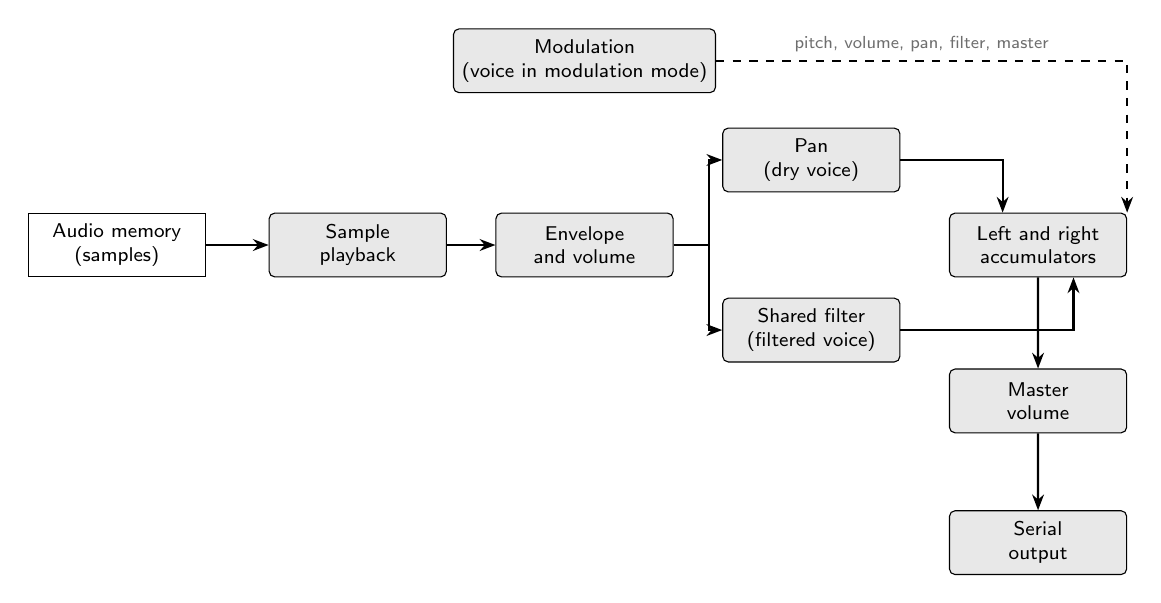
\begin{tikzpicture}[
			scale=0.9, transform shape,
			block/.style={draw, rounded corners=2pt, fill=sirclightgray, align=center, font=\footnotesize, minimum height=0.9cm, minimum width=2.5cm},
			store/.style={draw, fill=white, align=center, font=\footnotesize, minimum height=0.9cm, minimum width=2.5cm},
			flow/.style={-{Stealth[length=2mm]}, thick},
			ctl/.style={-{Stealth[length=2mm]}, thick, dashed},
			note/.style={font=\scriptsize, text=sircgray}
		]
		\node[store] (ram) at (0,0) {Audio memory\\(samples)};
		\node[block] (pcm) at (3.4,0) {Sample\\playback};
		\node[block] (env) at (6.6,0) {Envelope\\and volume};
		\node[block] (pan) at (9.8,1.2) {Pan\\(dry voice)};
		\node[block] (flt) at (9.8,-1.2) {Shared filter\\(filtered voice)};
		\node[block] (acc) at (13.0,0) {Left and right\\accumulators};
		\node[block] (mst) at (13.0,-2.2) {Master\\volume};
		\node[block] (out) at (13.0,-4.2) {Serial\\output};
		\node[block] (mod) at (6.6,2.6) {Modulation\\(voice in modulation mode)};
		\draw[flow] (ram) -- (pcm);
		\draw[flow] (pcm) -- (env);
		\draw[flow] (env.east) -- ++(0.5,0) |- (pan.west);
		\draw[flow] (env.east) -- ++(0.5,0) |- (flt.west);
		\draw[flow] (pan.east) -| ([xshift=-0.5cm]acc.north);
		\draw[flow] (flt.east) -| ([xshift=0.5cm]acc.south);
		\draw[flow] (acc) -- (mst);
		\draw[flow] (mst) -- (out);
		\draw[ctl] (mod.east) -| node[above, near start, note]{pitch, volume, pan, filter, master} (acc.north east);
	\end{tikzpicture}
	\caption{The Voice Signal Path}
	\label{fig:signal-path}
\end{figure}

\section{Block Diagrams}
\label{sec:block-diagrams}

Figure~\ref{fig:block-system} shows the device as the CPU sees it: a register block and a window onto audio memory
behind one bus interface, a serial output, and one interrupt line. The audio memory is not on the CPU's bus. It is a
separate memory behind the device, and the device alone controls it; the CPU reaches it only through the device. The
device and its memory are described in Chapters~\ref{ch:package} and~\ref{ch:memory-map}.

\begin{figure}[H]
	\centering
	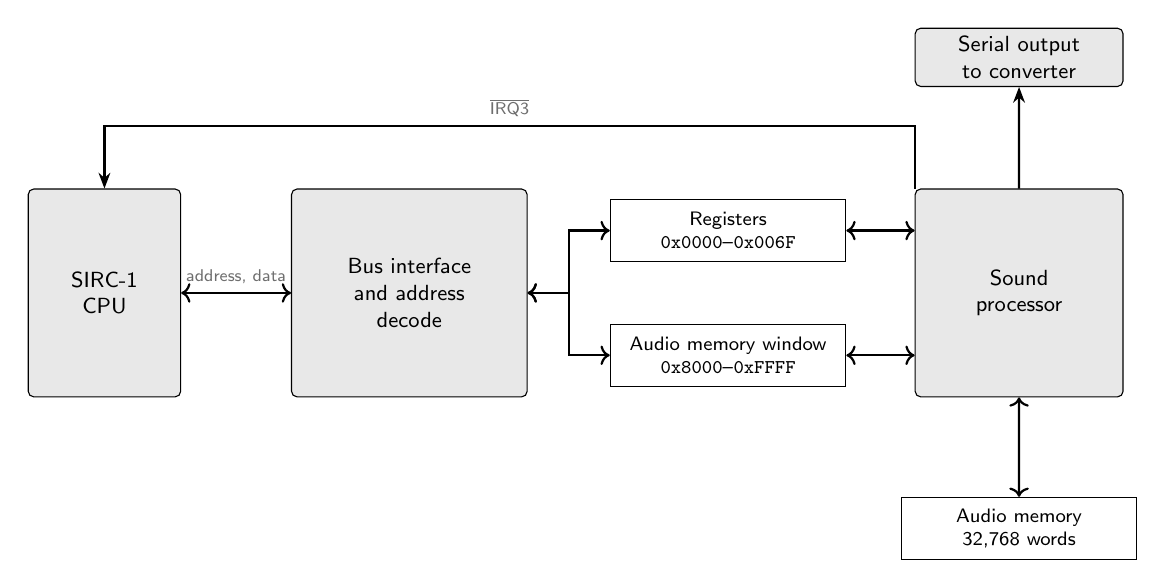
\begin{tikzpicture}[
			scale=0.88, transform shape,
			block/.style={draw, rounded corners=2pt, fill=sirclightgray, align=center, font=\small},
			mem/.style={draw, fill=white, align=center, font=\footnotesize, minimum height=0.9cm, minimum width=3.4cm},
			flow/.style={-{Stealth[length=2mm]}, thick},
			note/.style={font=\scriptsize, text=sircgray}
		]
		\node[block, minimum width=2.2cm, minimum height=3.0cm] (cpu) at (0,0) {SIRC-1\\CPU};
		\node[block, minimum width=3.4cm, minimum height=3.0cm] (bus) at (4.4,0) {Bus interface\\and address\\decode};
		\node[mem] (m1) at (9.0,0.9) {Registers\\\texttt{0x0000}--\texttt{0x006F}};
		\node[mem] (m2) at (9.0,-0.9) {Audio memory window\\\texttt{0x8000}--\texttt{0xFFFF}};
		\node[block, minimum width=3.0cm, minimum height=3.0cm] (snd) at (13.2,0) {Sound\\processor};
		\node[mem] (sram) at (13.2,-3.4) {Audio memory\\32,768 words};
		\node[block, minimum width=3.0cm] (dac) at (13.2,3.4) {Serial output\\to converter};
		\draw[flow, <->] (cpu) -- node[above, note]{address, data} (bus);
		\draw[flow, <->] (bus.east) -- ++(0.6,0) |- (m1.west);
		\draw[flow, <->] (bus.east) -- ++(0.6,0) |- (m2.west);
		\draw[flow, <->] (m1.east) -- (m1.east -| snd.west);
		\draw[flow, <->] (m2.east) -- (m2.east -| snd.west);
		\draw[flow, <->] (snd) -- (sram);
		\draw[flow] (snd) -- (dac);
		\draw[flow] (snd.north west) -- ++(0,0.9) -| node[above, near start, note]{\activelow{IRQ3}} (cpu.north);
	\end{tikzpicture}
	\caption{The Sound Device in the System}
	\label{fig:block-system}
\end{figure}

Figure~\ref{fig:block-spu} shows what is inside. One slot scheduler decides, in a fixed pattern, whether the audio
memory is used by the sound processor or by the CPU's window (Chapter~\ref{ch:timing}). The sound processor uses its
slots for sample reads first, and for the sequencers' instruction, instrument and pitch-table reads with what is left.

\begin{figure}[H]
	\centering
	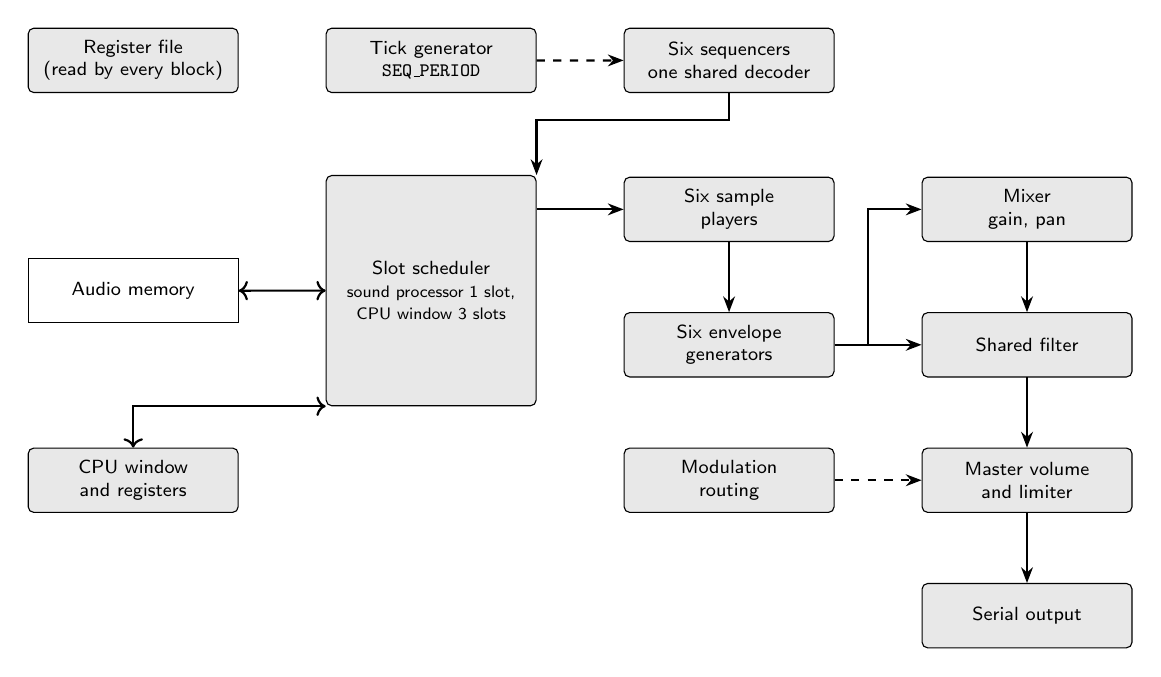
\begin{tikzpicture}[
			scale=0.86, transform shape,
			block/.style={draw, rounded corners=2pt, fill=sirclightgray, align=center, font=\footnotesize, minimum height=0.95cm, minimum width=3.1cm},
			store/.style={draw, fill=white, align=center, font=\footnotesize, minimum height=0.95cm, minimum width=3.1cm},
			flow/.style={-{Stealth[length=2mm]}, thick},
			ctl/.style={-{Stealth[length=2mm]}, thick, dashed},
			note/.style={font=\scriptsize, text=sircgray}
		]
		\node[block] (regs) at (0,6.6) {Register file\\(read by every block)};
		\node[block] (tick) at (4.4,6.6) {Tick generator\\\texttt{SEQ\_PERIOD}};
		\node[block] (seq) at (8.8,6.6) {Six sequencers\\one shared decoder};
		\node[store] (sram) at (0,3.2) {Audio memory};
		\node[block, minimum height=3.4cm] (arb) at (4.4,3.2) {Slot scheduler\\\scriptsize sound processor 1 slot,\\\scriptsize CPU window 3 slots};
		\node[block] (pcm) at (8.8,4.4) {Six sample\\players};
		\node[block] (env) at (8.8,2.4) {Six envelope\\generators};
		\node[block] (mod) at (8.8,0.4) {Modulation\\routing};
		\node[block] (mix) at (13.2,4.4) {Mixer\\gain, pan};
		\node[block] (flt) at (13.2,2.4) {Shared filter};
		\node[block] (mst) at (13.2,0.4) {Master volume\\and limiter};
		\node[block] (ser) at (13.2,-1.6) {Serial output};
		\node[block] (cpu) at (0,0.4) {CPU window\\and registers};
		\draw[ctl] (tick) -- (seq);
		\draw[flow, <->] (sram) -- (arb);
		\draw[flow, <->] (cpu) |- (arb.south west);
		\draw[flow] (arb.east |- pcm) -- (pcm.west);
		\draw[flow] (seq.south) -- ++(0,-0.4) -| (arb.north east);
		\draw[flow] (pcm.south) -- (env.north);
		\draw[flow] (env.east) -- ++(0.5,0) |- (mix.west);
		\draw[flow] (env.east) -- ++(0.5,0) |- (flt.west);
		\draw[flow] (mix.south) -- (flt.north);
		\draw[flow] (flt.south) -- (mst.north);
		\draw[flow] (mst.south) -- (ser.north);
		\draw[ctl] (mod.east) -- (mod.east -| mst.west);
	\end{tikzpicture}
	\caption{Blocks of the Sound Processor}
	\label{fig:block-spu}
\end{figure}

\section{Conventions}

\begin{itemize}
	\item Register and window addresses are in 16-bit words, as on the CPU. A word address is an offset from the base of the
	      device's segment unless stated otherwise. Sample data and some fields of the instrument table are byte offsets into
	      audio memory; each is marked where it occurs (Section~\ref{sec:byte-offsets}).
	\item Bit 0 is the least significant bit. Bit diagrams draw the most significant bit on the left.
	\item Hexadecimal values carry a \texttt{0x} prefix and upper case digits.
	\item Ranges of values and addresses use an en dash: \texttt{0x0000}--\texttt{0x00FF}.
	\item \textbf{Reserved} fields and registers are set aside by the architecture. Software must not rely on what they
	      read, and should write zero to a reserved field it does not otherwise use.
	\item A value that the design has not fixed is \textbf{not yet specified}. It is not undefined, and no value is implied.
	\item Fixed-point numbers are written $m.n$: $m$ integer bits and $n$ fraction bits. The position and step of a voice are
	      16.16 values, so their integer part is the high 16 bits.
	\item The \textbf{device} is the whole package, SIRCAS. It contains the \textbf{sound processor}, which is the six voices,
	      the mixer and the filter, together with the registers, the sequencers and the memory slot scheduler.
	\item A \textbf{tick} is one step of the sequencers' clock, whose period is set by \texttt{SEQ\_PERIOD}
	      (Chapter~\ref{ch:sequencer}). An \textbf{envelope update} is one step of a voice's envelope, made once in every 64
	      output samples (Chapter~\ref{ch:envelope}); portamento steps on it too.
	\item \textbf{Architecturally undefined} means that the manual does not say what the device does: the result may differ
	      between devices and between runs, and software must not depend on it. It is not the same as \textbf{not yet
		      specified}, which marks a decision the design has still to make, nor as the contents of audio memory at reset, which
	      are \textbf{undefined} until the program writes them.
	\item In formulas, $\ll$ and $\gg$ are shifts left and right (a right shift of a negative number rounds towards minus
	      infinity), $\lfloor x \rfloor$ rounds down, $\lceil x \rceil$ rounds up, and $a \bmod b$ is the remainder of $a$
	      divided by $b$.
\end{itemize}

\chapter{Package and Pinout}
\label{ch:package}

The sound device is a single integrated circuit with a memory of its own attached. The sound processor, the registers
and the slot scheduler are on the one piece of silicon. The audio memory is a separate static memory that the device
alone controls, and it is not on the CPU's bus. The signals that leave the package are therefore the bus, one interrupt
output, the clock and reset inputs, the memory interface, and the serial output for the converter. This chapter gives
the groups of signals and the meaning of each. Chapter~\ref{ch:signal-timing} gives the timing of the signals.

\section{Package}

The package and the pin numbers are not yet specified. The device has 77 signal pins, listed in
Table~\ref{tab:signals}, in addition to its power and ground pins, whose number is also not yet specified.

\section{Signal Groups}

Figure~\ref{fig:signal-groups} shows the signals by group. Three groups face three neighbours: the CPU's bus, the audio
memory, and the converter.

\begin{figure}[H]
	\centering
	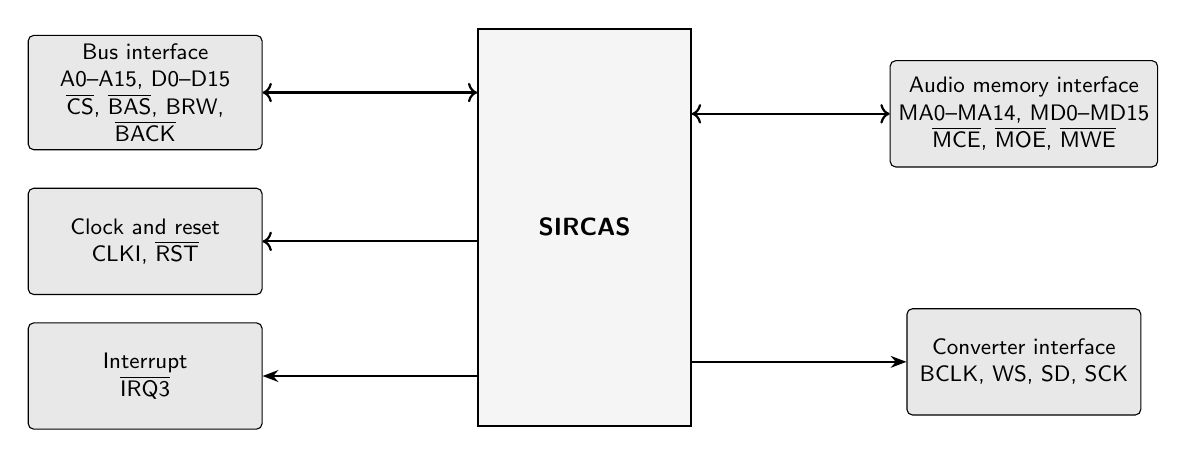
\begin{tikzpicture}[
			scale=0.9, transform shape,
			group/.style={draw, rounded corners=2pt, fill=sirclightgray, align=center, font=\small, minimum width=3.3cm, minimum height=1.5cm},
			chip/.style={draw, thick, fill=gray!8, align=center, font=\bfseries, minimum width=3.0cm, minimum height=5.6cm},
			flow/.style={-{Stealth[length=2mm]}, thick},
			note/.style={font=\scriptsize, text=sircgray, align=center}
		]
		\node[chip] (chip) at (0,0) {SIRCAS};
		\node[group] (bus) at (-6.2,1.9) {Bus interface\\A0--A15, D0--D15\\\activelow{CS}, \activelow{BAS}, BRW,\\\activelow{BACK}};
		\node[group] (clk) at (-6.2,-0.2) {Clock and reset\\CLKI, \activelow{RST}};
		\node[group] (irq) at (-6.2,-2.1) {Interrupt\\\activelow{IRQ3}};
		\node[group] (mem) at (6.2,1.6) {Audio memory interface\\MA0--MA14, MD0--MD15\\\activelow{MCE}, \activelow{MOE}, \activelow{MWE}};
		\node[group] (dac) at (6.2,-1.9) {Converter interface\\BCLK, WS, SD, SCK};
		\draw[flow, <->] (bus.east) -- (bus.east -| chip.west);
		\draw[flow, <-] (clk.east) -- (clk.east -| chip.west);
		\draw[flow] (chip.west |- irq) -- (irq.east);
		\draw[flow, <->] (chip.east |- mem) -- (mem.west);
		\draw[flow] (chip.east |- dac) -- (dac.west);
	\end{tikzpicture}
	\caption{SIRCAS Signal Groups}
	\label{fig:signal-groups}
\end{figure}

\section{Signal Descriptions}

Table~\ref{tab:signals} lists the direction and sense of each signal. Active-low signals carry a bar over the name;
they are asserted when low. Address, data and converter signals are active high. An output marked \emph{open drain} can
only pull its line low; the system supplies a pull-up, and several devices may share the line.

\begin{table}[H]
	\centering
	\small
	\begin{tabularx}{\textwidth}{llllX}
		\toprule
		\textbf{Signal}  & \textbf{Count} & \textbf{Direction} & \textbf{Output type} & \textbf{Function}                                              \\
		\midrule
		CLKI             & 1              & Input              &                      & Rising edge advances the device one cycle                      \\
		\activelow{RST}  & 1              & Input              &                      & Resets the device                                              \\
		\activelow{CS}   & 1              & Input              &                      & Selects the device for a bus cycle                             \\
		\activelow{BAS}  & 1              & Input              &                      & Marks a bus cycle                                              \\
		BRW              & 1              & Input              &                      & High for a read, low for a write                               \\
		\activelow{BACK} & 1              & Output             & Open drain           & Completes the bus cycle                                        \\
		A0--A15          & 16             & Input              &                      & Word offset in the device segment                              \\
		D0--D15          & 16             & Bidirectional      & Three-state          & Data                                                           \\
		\activelow{IRQ3} & 1              & Output             & Open drain           & A completed sequence is waiting (Section~\ref{sec:interrupts}) \\
		MA0--MA14        & 15             & Output             &                      & Word address of the audio memory                               \\
		MD0--MD15        & 16             & Bidirectional      & Three-state          & Audio memory data                                              \\
		\activelow{MCE}  & 1              & Output             &                      & Audio memory chip enable                                       \\
		\activelow{MOE}  & 1              & Output             &                      & Audio memory output enable                                     \\
		\activelow{MWE}  & 1              & Output             &                      & Audio memory write enable                                      \\
		BCLK             & 1              & Output             &                      & Serial bit clock to the converter                              \\
		WS               & 1              & Output             &                      & Serial word select: low for left, high for right               \\
		SD               & 1              & Output             &                      & Serial data                                                    \\
		SCK              & 1              & Output             &                      & Converter system clock                                         \\
		\bottomrule
	\end{tabularx}
	\caption{SIRCAS Signals}
	\label{tab:signals}
\end{table}

\subsection{Clock Input (CLKI)}

\textbf{Direction:} Input. The device is clocked by \texttt{CLKI}, a continuous clock of 10,738,636 Hz in an NTSC
system: half the frequency of the 21,477,272 Hz system oscillator. Every interval in this manual that is measured in
cycles is a count of \texttt{CLKI} cycles. The sample period is 336 cycles (Chapter~\ref{ch:timing}). The device
works at any steady frequency from 9.0 to 12.0~MHz (Section~\ref{sec:clock-rate}). In a PAL system \texttt{CLKI} is 10,640,685~Hz, half the 21,281,370~Hz system oscillator.

\subsection{Reset Input (RST)}

\textbf{Direction:} Input. \textbf{Signal Type:} Active Low. While \activelow{RST} is asserted
the device holds every register in its reset state (Section~\ref{sec:reset}). The audio memory is not cleared: its
contents are undefined after power-up and after reset.

\subsection{Bus Signals}

\activelow{BAS}, BRW, A0--A15, D0--D15 and \activelow{BACK} are bus signals of the SIRC-1, defined in the \hwmanual{}. \activelow{CS} is produced by the system's address decoding of the device's segment. A cycle is addressed to the device when \activelow{CS} and \activelow{BAS} are both
asserted. The address is a word offset in the device's 65,536-word segment (Chapter~\ref{ch:memory-map}). The device
asserts \activelow{BACK} to complete the cycle. Register accesses are completed without delay. An access to the audio
memory window is completed when the device has made it, which takes between two and five \texttt{CLKI} cycles
(Section~\ref{sec:cpu-slots}).

\subsection{Interrupt Output (IRQ3)}
\label{sec:pin-irq3}

\textbf{Direction:} Output. \textbf{Signal Type:} Active Low, open drain. The device holds \activelow{IRQ3} asserted
for as long as at least one sequence has completed whose interrupt is enabled (Section~\ref{sec:interrupts}). The
signal is level-sensitive. It is released when no enabled flag remains set.

\subsection{Audio Memory Interface (MA, MD, MCE, MOE, MWE)}
\label{sec:memory-interface}

The audio memory is 32,768 words of 16 bits, so it has a 15-bit address and a 16-bit data bus. It may be built from two
32,768 by 8 bit memories used side by side. The memory interface belongs to the sound device alone: the CPU's bus and
the memory's bus are separate, and the device is the only user of the memory. The device makes every access, both its
own and the CPU's (Section~\ref{sec:cpu-slots}), in a fixed pattern of slots, so the CPU is never in competition with
the sound processor for the memory.

Every memory transaction, a read or a write, occupies two \texttt{CLKI} cycles, which is 186 ns. The memory must
therefore complete an access within two cycles. The electrical figures of the interface are in
Section~\ref{sec:electrical}; the timing of \activelow{MCE}, \activelow{MOE} and \activelow{MWE} within an access is
not yet specified.

\subsection{Converter Interface (BCLK, WS, SD, SCK)}
\label{sec:converter-interface}

The device is the master of the serial interface to the converter. It sends the two stereo channels time-multiplexed on
\texttt{SD}, with \texttt{WS} low for the left channel and high for the right, and \texttt{BCLK} clocking the bits
(Chapter~\ref{ch:signal-timing}). \texttt{SCK} is a clock for converters that need a system clock in addition to the
bit clock; its frequency and phase relation to \texttt{BCLK} are not yet specified.

\section{Electrical Characteristics}
\label{sec:electrical}

The figures in this section are provisional. They are targets the device is designed to meet, and will be confirmed or
revised when it is characterised. They are the same as those of the CPU (\hwmanual{}, electrical characteristics
chapter), so that the three devices fit together on one bus. The supply is 5~V $\pm$ 5\%, the signals are TTL
compatible, and all figures apply over 0 to 70~\textdegree{}C. Times are measured from or to the 1.4~V point of the
rising edge of \texttt{CLKI}, with the outputs loaded by 50~pF.

\begin{table}[H]
	\centering
	\begin{tabular}{p{7.6cm}lrrl}
		\toprule
		\textbf{Parameter}                                                                         & \textbf{Symbol}    & \textbf{Min} & \textbf{Max} & \textbf{Unit} \\
		\midrule
		\texttt{CLKI} frequency                                                                    & $f_{CLKI}$         & 9.0          & 12.0         & MHz           \\
		\texttt{CLKI} high time and low time                                                       & $t_{CH}$, $t_{CL}$ & 35           &              & ns            \\
		Input high voltage, input low voltage                                                      &                    & 2.0, 0       & VCC, 0.8     & V             \\
		Output high voltage ($I_{OH} = -400~\mu$A), output low voltage ($I_{OL} = 4$~mA)           &                    & 2.4          & 0.4          & V             \\
		Low level of an open-drain output, $I_{OL} = 8$~mA                                         &                    &              & 0.4          & V             \\
		Input capacitance                                                                          &                    &              & 10           & pF            \\
		\midrule
		Bus inputs (A, D on a write, BRW, \activelow{CS}, \activelow{BAS}): set-up before the edge & $t_{IS}$           & 10           &              & ns            \\
		Bus inputs: hold after the edge                                                            & $t_{IH}$           & 0            &              & ns            \\
		Read data and \activelow{BACK} valid after \activelow{CS} and \activelow{BAS} asserted     & $t_{AV}$           &              & 35           & ns            \\
		Read data float, after the edge that ends a read                                           & $t_{OZ}$           &              & 25           & ns            \\
		Output hold                                                                                & $t_{OH}$           & 3            &              & ns            \\
		\bottomrule
	\end{tabular}
	\caption{AC and DC Characteristics}
	\label{tab:electrical}
\end{table}

\noindent The memory interface outputs (MA, MCE, MOE, MWE and MD on a write) are valid within 25~ns of the edge that starts the access, and are held for 3~ns, and the read data has 10~ns of set-up before the edge that ends it, with no hold. An access takes two cycles, 186~ns, so the memory's address access time may be at most 140~ns, with 5~ns left for the board. At 12~MHz an access is 167~ns and the limit is 120~ns.

\chapter{Memory Map and Bus Access}
\label{ch:memory-map}

\section{The Device Segment}

The sound device occupies one segment of the CPU's address space, 65,536 words long. The segment is chosen by the
system; the segment that the SIRCUS system uses is not yet specified. This manual gives every address as an offset from
the base of the segment.

\begin{table}[H]
	\centering
	\begin{tabular}{llp{6.5cm}}
		\toprule
		\textbf{Offsets}                 & \textbf{Region}     & \textbf{Notes}                                                                    \\
		\midrule
		\texttt{0x0000}--\texttt{0x000F} & Global registers    & Offsets \texttt{0x0000}--\texttt{0x000B} are defined (Chapter~\ref{ch:registers}) \\
		\texttt{0x0010}--\texttt{0x001F} & Voice 0 registers   & Eight registers defined (Section~\ref{sec:voice-registers})                       \\
		\texttt{0x0020}--\texttt{0x002F} & Voice 1 registers   & As voice 0                                                                        \\
		\texttt{0x0030}--\texttt{0x003F} & Voice 2 registers   & As voice 0                                                                        \\
		\texttt{0x0040}--\texttt{0x004F} & Voice 3 registers   & As voice 0                                                                        \\
		\texttt{0x0050}--\texttt{0x005F} & Voice 4 registers   & As voice 0                                                                        \\
		\texttt{0x0060}--\texttt{0x006F} & Voice 5 registers   & As voice 0                                                                        \\
		\texttt{0x0070}--\texttt{0x7FFF} & Reserved            & Reads zero, writes ignored                                                        \\
		\texttt{0x8000}--\texttt{0xFFFF} & Audio memory window & 32,768 words (Section~\ref{sec:audio-memory})                                     \\
		\bottomrule
	\end{tabular}
	\caption{Sound Device Memory Map}
	\label{tab:memory-map}
\end{table}

The \textbf{registers} control the device. The global registers are at offsets \texttt{0x0000}--\texttt{0x000F}. Each
of the six voices has a block of 16 registers, at \texttt{0x0010} plus 16 times the voice number. They are described in
Chapter~\ref{ch:registers}.

\section{The Audio Memory}
\label{sec:audio-memory}

The audio memory holds everything the voices play and everything that controls them: sample data, the instrument table,
the pitch tables and the sequences. It is 32,768 words, which is 64 KB. The device does not interpret the memory in any
fixed layout. Registers and instrument fields hold the addresses of the things they use, and any range of the memory
may hold any of them.

The CPU reaches the memory through the window at offsets \texttt{0x8000}--\texttt{0xFFFF}. The offset \texttt{0x8000}
plus $n$ selects word $n$ of the memory. The memory is not on the CPU's bus, and the CPU has no other way to reach it
(Section~\ref{sec:memory-interface}).

\subsection{Word and Byte Addresses}
\label{sec:byte-offsets}

Two kinds of address name the same memory, and a field says which it holds:

\begin{itemize}
	\item A \textbf{window address} is the CPU's word address of a word: \texttt{0x8000} for the first word, \texttt{0xFFFF} for
	      the last. \texttt{INSTR\_BASE} and \texttt{SEQ\_PC} hold window addresses.
	\item A \textbf{byte offset} is a count of bytes from the start of the audio memory, \texttt{0x0000}--\texttt{0xFFFF}. The
	      sample start, the pitch table address and the loop start of an instrument are byte offsets, as are the sample position
	      of a voice and its length. The byte at offset $b$ is in the word at window address $\texttt{0x8000} + \lfloor b/2
		      \rfloor$.
\end{itemize}

The sequencer's \texttt{GOTO} displacement is a count of instruction words (Chapter~\ref{ch:sequencer}).

\subsection{Byte Order}
\label{sec:byte-order}

A word holds two bytes, and the byte at the even offset is the high byte. For the word \texttt{0x1234}, the byte at an
even offset is \texttt{0x12} (bits 15--8) and the byte at the next odd offset is \texttt{0x34} (bits 7--0). Sample
bytes are signed two's-complement values. Multi-byte values in the tables of Chapter~\ref{ch:formats} are stored with
the high word first.

\section{Access Rules}
\label{sec:access-rules}

A read of a register, a reserved offset or a word of the window returns the stored value, or zero for a reserved
offset. A write stores the value, or is ignored at a reserved offset. No register has a side effect on a read. The
registers that act on a write are described with their registers (Chapter~\ref{ch:registers}).

\begin{itemize}
	\item \textbf{Registers} are accessed without delay: the device completes the cycle at once. A register access never
	      waits for the audio memory.
	\item \textbf{The window} is accessed in the device's memory schedule (Chapter~\ref{ch:timing}). A window access
	      is held until one of the slots reserved for the CPU comes round, and takes between two and five cycles to
	      complete, whatever the voices and sequencers are doing.
	\item \textbf{Playing and the window.} The CPU may read and write the audio memory while the voices play. The sound
	      processor reads in the first slot of each pattern of four slots and the CPU's window uses the other three, so a
	      read by the sound processor sees every write by the CPU that completed before its slot began. A program that
	      rewrites a word a voice is reading must not depend on whether the old or the new value is read for the one sample
	      in which the two coincide.
\end{itemize}

At reset the contents of the audio memory are undefined. A program must write every word it uses before it starts a
voice or a sequence that uses it (Section~\ref{sec:startup}).

\section{Planning an Audio Memory Layout}
\label{sec:layout}

Nothing fixes where the tables live, so a program chooses. One arrangement puts the instrument table at the start of
the memory, then the pitch tables, then the sequences, and gives the rest to sample data:

\begin{table}[H]
	\centering
	\begin{tabular}{lll}
		\toprule
		\textbf{Contents}                       & \textbf{Window addresses}  & \textbf{Size}                     \\
		\midrule
		Instrument table (\texttt{INSTR\_BASE}) & \texttt{0x8000} and up     & 8 words (16 bytes) per instrument \\
		Pitch tables                            & after the instrument table & 24 words (48 bytes) per table     \\
		Sequences                               & after the pitch tables     & One word per instruction          \\
		Sample data                             & the rest                   & One byte per sample               \\
		\bottomrule
	\end{tabular}
	\caption{An Example Audio Memory Layout}
	\label{tab:layout}
\end{table}

A sample takes one byte per sample point, so the whole memory holds at most about two seconds of sound at the device's
output rate if it is played at its original pitch with one sample point per output sample. Looping a short waveform
repeats its bytes, so a looped voice uses very little memory (Chapter~\ref{ch:playback}).

\chapter{Registers}
\label{ch:registers}

\section{Register Map}

The registers occupy the first words of the device segment. Every defined register is 16 bits wide and is read and
written a word at a time. The global registers are at offsets \texttt{0x0000}--\texttt{0x000F}; each voice has 16
registers starting at \texttt{0x0010} plus 16 times the voice number.

\begin{table}[H]
	\centering
	\begin{tabular}{lllp{6.2cm}}
		\toprule
		\textbf{Offset}                  & \textbf{Name}              & \textbf{Access} & \textbf{Description}                                             \\
		\midrule
		\texttt{0x0000}                  & \texttt{CONFIG}            & R/W             & Audio enable                                                     \\
		\texttt{0x0001}                  & \texttt{STATUS}            & R               & Version, sequence interrupt, memory overrun                      \\
		\texttt{0x0002}                  & \texttt{STATUSCLR}         & W               & Clears the memory overrun flag                                   \\
		\texttt{0x0003}                  & \texttt{SEQ\_PERIOD}       & R/W             & Output samples per sequencer tick; 0 stops the ticks             \\
		\texttt{0x0004}                  & \texttt{SEQ\_DONE}         & R, W1C          & Sequence completion flags, one per voice                         \\
		\texttt{0x0005}                  & \texttt{SEQ\_INT\_EN}      & R/W             & Sequence completion interrupt enables                            \\
		\texttt{0x0006}                  & \texttt{INSTR\_BASE}       & R/W             & Window address of the instrument table                           \\
		\texttt{0x0007}                  & \texttt{MASTER\_VOL}       & R/W             & Master volume                                                    \\
		\texttt{0x0008}                  & \texttt{FILTER\_CONFIG}    & R/W             & Filter output: low-pass, band-pass or high-pass                  \\
		\texttt{0x0009}                  & \texttt{FILTER\_CUTOFF}    & R/W             & Filter cutoff                                                    \\
		\texttt{0x000A}                  & \texttt{FILTER\_RESONANCE} & R/W             & Filter resonance                                                 \\
		\texttt{0x000B}                  & \texttt{FILTER\_VOL\_PAN}  & R/W             & Filter output volume and pan                                     \\
		\texttt{0x000C}--\texttt{0x000F} & ---                        & Reserved        & Reads zero, writes ignored                                       \\
		\midrule
		\multicolumn{4}{l}{\textit{Voice registers, at the voice base: \texttt{0x0010} + 16 $\times$ voice}}                                               \\
		\midrule
		base + 0                         & \texttt{CONTROL}           & R/W             & Sequencer enable, routing, portamento                            \\
		base + 1                         & \texttt{VOLUME\_PAN}       & R/W             & Volume and pan                                                   \\
		base + 2                         & \texttt{MOD\_ROUTE}        & R/W             & Modulation destination                                           \\
		base + 3                         & \texttt{INSTR}             & R/W             & Instrument selected for the next note                            \\
		base + 4                         & \texttt{FINE}              & R/W             & Fine pitch adjustment                                            \\
		base + 5                         & \texttt{PORTA\_RATE}       & R/W             & Portamento rate                                                  \\
		base + 6                         & \texttt{COMMAND}           & W               & Direct note or stop                                              \\
		base + 7                         & \texttt{SEQ\_PC}           & R/W             & Sequencer program counter; a write restarts the voice's sequence \\
		base + 8--15                     & ---                        & Reserved        & Reads zero, writes ignored                                       \\
		\bottomrule
	\end{tabular}
	\caption{Register Map}
	\label{tab:register-map}
\end{table}

\emph{W1C} means that writing a 1 to a bit clears it and writing a 0 leaves it unchanged. The names are those of this
manual. A voice register for voice $n$ is at \texttt{0x0010} $+ 16n +$ its offset in the voice block.

\section{Global Registers}

\subsection{Configuration Register}
\label{sec:reg-config}

\begin{figure}[H]
	\centering
	\begin{bytefield}[bitwidth=2em]{16}
		\bitheader{0-15} \\
		\bitbox{1}{\footnotesize EN} &
		\bitbox{15}{Reserved}
	\end{bytefield}
	\caption{Configuration Register (\texttt{CONFIG}, Offset \texttt{0x0000})}
	\label{fig:reg-config}
\end{figure}

\begin{table}[H]
	\centering
	\begin{tabular}{llp{8.0cm}}
		\toprule
		\textbf{Bits} & \textbf{Field}     & \textbf{Meaning}                                                                                            \\
		\midrule
		15            & \texttt{AUDIO\_EN} & Audio enable: when 0 both converter channels are forced to digital zero; when 1 the mix is sent. 0 at reset \\
		14--0         & ---                & Reserved: reads zero, writes ignored                                                                        \\
		\bottomrule
	\end{tabular}
	\caption{Configuration Register Fields}
	\label{tab:reg-config-fields}
\end{table}

In Figure~\ref{fig:reg-config}, EN is \texttt{AUDIO\_EN}. \texttt{AUDIO\_EN} gates the output only. While it is 0 the
device runs exactly as it does when it is 1: envelopes advance, sample positions move, modulation and the filter run,
and the sequencers keep time. Clearing and setting it mutes and unmutes without changing any of that.

\subsection{Status and Status Clear Registers}
\label{sec:reg-status}

\begin{figure}[H]
	\centering
	\begin{bytefield}[bitwidth=2em]{16}
		\bitheader{0-15} \\
		\bitbox{10}{Reserved (reads zero)} &
		\bitbox{1}{\footnotesize OVR} &
		\bitbox{1}{\footnotesize IRQ} &
		\bitbox{4}{VERSION}
	\end{bytefield}
	\caption{Status Register (\texttt{STATUS}, Offset \texttt{0x0001})}
	\label{fig:reg-status}
\end{figure}

\begin{table}[H]
	\centering
	\begin{tabular}{llp{8.0cm}}
		\toprule
		\textbf{Bits} & \textbf{Field}        & \textbf{Meaning}                                                                                                                                                                \\
		\midrule
		15--6         & ---                   & Reads zero                                                                                                                                                                      \\
		5             & \texttt{MEM\_OVERRUN} & A memory deadline was missed: a sample read, or the sequencer work of a tick (Section~\ref{sec:deadlines}). Set by the device and held until cleared through \texttt{STATUSCLR} \\
		4             & \texttt{SEQ\_IRQ}     & 1 while \activelow{IRQ3} is asserted: at least one \texttt{SEQ\_DONE} flag is set and enabled in \texttt{SEQ\_INT\_EN}                                                          \\
		3--0          & \texttt{VERSION}      & Device revision, 1                                                                                                                                                              \\
		\bottomrule
	\end{tabular}
	\caption{Status Register Fields}
	\label{tab:reg-status-fields}
\end{table}

In Figure~\ref{fig:reg-status}, OVR is \texttt{MEM\_OVERRUN} and IRQ is \texttt{SEQ\_IRQ}. \texttt{STATUS} is
read-only; a write to its offset is ignored. A write to \texttt{STATUSCLR} (offset \texttt{0x0002}) with bit 5 set
clears \texttt{MEM\_OVERRUN}; the other bits are ignored, and the register reads zero.

\subsection{Sequencer Registers}
\label{sec:reg-sequencer}

\texttt{SEQ\_PERIOD} (offset \texttt{0x0003}) is an unsigned 16-bit count of output samples per sequencer tick.
Zero stops the ticks. A tick of 666 samples, for example, is about 20.84 ms. A write restarts the count towards the
next tick (Chapter~\ref{ch:sequencer}).

\texttt{SEQ\_DONE} (offset \texttt{0x0004}) holds one sticky flag for each voice, in bits 5--0 (bit $n$ belongs to voice $n$): the device sets a voice's
flag when its sequence ends (Section~\ref{sec:seq-end}). Reading the register does not clear a flag. Writing a 1 to a
bit clears that flag; so does a write to the voice's \texttt{SEQ\_PC}. Bits 15--6 read zero.

\texttt{SEQ\_INT\_EN} (offset \texttt{0x0005}) holds one interrupt enable for each voice, in bits 5--0 (bit $n$ for voice $n$). Bits 15--6 read
zero. Disabling an interrupt never clears a flag. \activelow{IRQ3} is asserted whenever any bit of
\texttt{SEQ\_DONE} and the same bit of \texttt{SEQ\_INT\_EN} are both 1 (Section~\ref{sec:interrupts}).

\subsection{Instrument Base Register}

\texttt{INSTR\_BASE} (offset \texttt{0x0006}) holds the window address (\texttt{0x8000}--\texttt{0xFFFF}) of the first word
of the instrument table (Section~\ref{sec:instrument-table}). Instrument $i$ is at \texttt{INSTR\_BASE} $+ 8i$.

\subsection{Master Volume Register}

\texttt{MASTER\_VOL} (offset \texttt{0x0007}) holds an unsigned 8-bit gain in bits 7--0; bits 15--8 read zero. The mixer
multiplies each output channel by the value and divides by 256 (Section~\ref{sec:master-volume}). The reset value is
255.

\subsection{Filter Registers}
\label{sec:reg-filter}

\begin{figure}[H]
	\centering
	\begin{bytefield}[bitwidth=2em]{16}
		\bitheader{0-15} \\
		\bitbox{8}{Volume} &
		\bitbox{8}{Pan}
	\end{bytefield}
	\caption{Filter Volume and Pan Register (\texttt{FILTER\_VOL\_PAN}, Offset \texttt{0x000B})}
	\label{fig:reg-filter-vol-pan}
\end{figure}

\begin{table}[H]
	\centering
	\begin{tabular}{llp{7.5cm}}
		\toprule
		\textbf{Offset} & \textbf{Register}          & \textbf{Meaning}                                                                                           \\
		\midrule
		\texttt{0x0008} & \texttt{FILTER\_CONFIG}    & Bits 1--0 select the output: 00 low-pass, 01 band-pass, 10 high-pass; 11 is reserved. Other bits read zero \\
		\texttt{0x0009} & \texttt{FILTER\_CUTOFF}    & Unsigned 8-bit cutoff coefficient in bits 7--0 (Section~\ref{sec:filter-cutoff})                           \\
		\texttt{0x000A} & \texttt{FILTER\_RESONANCE} & Unsigned 8-bit resonance in bits 7--0 (Section~\ref{sec:filter-resonance})                                 \\
		\texttt{0x000B} & \texttt{FILTER\_VOL\_PAN}  & Filter output volume in bits 15--8, pan in bits 7--0 (Section~\ref{sec:filter-output})                     \\
		\bottomrule
	\end{tabular}
	\caption{Filter Registers}
	\label{tab:reg-filter}
\end{table}

There is no register bit that turns the filter off. A voice reaches the filter or avoids it by its own routing bit
(Section~\ref{sec:reg-control}).

\subsection{Reset State}
\label{sec:reset}

At reset the device is silent: \texttt{AUDIO\_EN} is 0, so the converter receives digital zero until the program sets
it. The sample generator and the memory scheduler run from reset, muted or not.

\begin{table}[H]
	\centering
	\begin{tabular}{ll}
		\toprule
		\textbf{Item}                                                   & \textbf{State at reset} \\
		\midrule
		\texttt{CONFIG}                                                 & 0                       \\
		\texttt{MASTER\_VOL}                                            & 255                     \\
		\texttt{SEQ\_PERIOD}, \texttt{SEQ\_DONE}, \texttt{SEQ\_INT\_EN} & 0                       \\
		\texttt{MEM\_OVERRUN}                                           & 0                       \\
		Each voice's \texttt{CONTROL}                                   & 0                       \\
		Each voice's volume                                             & 0                       \\
		Each voice's pan                                                & 128                     \\
		Envelopes, playback and modulation                              & Inactive                \\
		Each sequencer's \texttt{WAIT} counter and \texttt{END} counter & 0                       \\
		The filter state                                                & Zero                    \\
		Audio memory                                                    & Undefined               \\
		Every other register                                            & Not yet specified       \\
		\bottomrule
	\end{tabular}
	\caption{State at Reset}
	\label{tab:reset}
\end{table}

A program writes every register it relies on before it starts a voice (Section~\ref{sec:startup}).

\section{Voice Registers}
\label{sec:voice-registers}

\subsection{Control Register}
\label{sec:reg-control}

\begin{figure}[H]
	\centering
	\begin{bytefield}[bitwidth=2em]{16}
		\bitheader{0-15} \\
		\bitbox{1}{\footnotesize SEQ} &
		\bitbox{1}{\footnotesize MOD} &
		\bitbox{1}{\footnotesize FLT} &
		\bitbox{1}{\footnotesize POR} &
		\bitbox{12}{Reserved}
	\end{bytefield}
	\caption{Voice Control Register (\texttt{CONTROL}, Voice Offset 0)}
	\label{fig:reg-control}
\end{figure}

\begin{table}[H]
	\centering
	\begin{tabular}{llp{8.0cm}}
		\toprule
		\textbf{Bits} & \textbf{Field}      & \textbf{Meaning}                                                                                                              \\
		\midrule
		15            & \texttt{SEQ\_EN}    & Sequencer enable: the voice's sequencer runs. When 0 the CPU controls the voice directly (Section~\ref{sec:direct-control})   \\
		14            & \texttt{MOD\_MODE}  & Modulation source: the voice makes no sound and steers a parameter (Chapter~\ref{ch:modulation})                              \\
		13            & \texttt{FILTER\_EN} & Filtered: the voice goes to the filter input instead of the dry mix                                                           \\
		12            & \texttt{PORTA\_EN}  & Portamento: a note on the instrument that the voice is already playing glides to the new pitch (Section~\ref{sec:portamento}) \\
		11--0         & ---                 & Reserved                                                                                                                      \\
		\bottomrule
	\end{tabular}
	\caption{Voice Control Register Fields}
	\label{tab:reg-control-fields}
\end{table}

In Figure~\ref{fig:reg-control}, SEQ, MOD, FLT and POR are \texttt{SEQ\_EN}, \texttt{MOD\_MODE}, \texttt{FILTER\_EN}
and \texttt{PORTA\_EN}. \texttt{MOD\_MODE} takes precedence over \texttt{FILTER\_EN}: a voice in modulation mode is in
neither mix. Changing \texttt{SEQ\_EN} does not start, stop or restart anything. A voice that was playing keeps
playing, and a sequence keeps its program counter.

\subsection{Volume and Pan Register}

\begin{figure}[H]
	\centering
	\begin{bytefield}[bitwidth=2em]{16}
		\bitheader{0-15} \\
		\bitbox{8}{Volume} &
		\bitbox{8}{Pan}
	\end{bytefield}
	\caption{Voice Volume and Pan Register (\texttt{VOLUME\_PAN}, Voice Offset 1)}
	\label{fig:reg-volume-pan}
\end{figure}

Bits 15--8 are the voice's volume, unsigned: 0 is silent. Bits 7--0 are its pan: 0 is the left channel only, 128 is
centre and 255 is almost entirely the right channel (Section~\ref{sec:mixing}). The reset volume is 0 and the reset pan
is 128. A volume or pan that a modulation voice is steering changes the value in force, not the value in the register
(Chapter~\ref{ch:modulation}).

\subsection{Modulation Route Register}
\label{sec:reg-mod-route}

\begin{figure}[H]
	\centering
	\begin{bytefield}[bitwidth=2em]{16}
		\bitheader{0-15} \\
		\bitbox{3}{DEST} &
		\bitbox{3}{VOICE} &
		\bitbox{4}{SHIFT} &
		\bitbox{1}{\footnotesize INV} &
		\bitbox{5}{Reserved}
	\end{bytefield}
	\caption{Modulation Route Register (\texttt{MOD\_ROUTE}, Voice Offset 2)}
	\label{fig:reg-mod-route}
\end{figure}

\begin{table}[H]
	\centering
	\begin{tabular}{llp{8cm}}
		\toprule
		\textbf{Bits} & \textbf{Field} & \textbf{Meaning}                                                                                                  \\
		\midrule
		15--13        & \texttt{DEST}  & Destination: 0 off, 1 pitch, 2 volume, 3 pan, 4 filter cutoff, 5 master volume, 6 filter pan; 7 reserved          \\
		12--10        & \texttt{VOICE} & Destination voice, 0--5, for the destinations that belong to a voice (pitch, volume, pan); ignored for the others \\
		9--6          & \texttt{SHIFT} & Signed 4-bit scale exponent, $-8$ to $+7$                                                                         \\
		5             & \texttt{INV}   & Invert the modulation value                                                                                       \\
		4--0          & ---            & Reserved                                                                                                          \\
		\bottomrule
	\end{tabular}
	\caption{Modulation Route Register Fields}
	\label{tab:reg-mod-route-fields}
\end{table}

The register takes effect only while the voice's \texttt{MOD\_MODE} is 1 (Chapter~\ref{ch:modulation}).

\subsection{Instrument and Fine Registers}

\texttt{INSTR} (voice offset 3) holds the number of the instrument the voice's next note uses, in bits 7--0; bits 15--8
read zero. \texttt{FINE} (voice offset 4) holds a signed 13-bit pitch adjustment in bits 12--0. A read of \texttt{FINE}
returns the value sign-extended to 16 bits. Both are set by the sequencer's \texttt{INST} and \texttt{FINE}
instructions, or by the CPU while \texttt{SEQ\_EN} is 0. While \texttt{SEQ\_EN} is 1, a CPU write to either is
discarded.

\subsection{Portamento Rate Register}

\texttt{PORTA\_RATE} (voice offset 5) is an unsigned 16-bit rate: how far the step moves at each envelope update, in raw units of the 16.16 step, where one unit is 1/65,536 of a sample byte per output sample. An envelope update is made every 64 output samples, 2.0 ms (Section~\ref{sec:portamento}). Zero holds the current pitch.

\subsection{Command Register}
\label{sec:reg-command}

\begin{figure}[H]
	\centering
	\begin{bytefield}[bitwidth=2em]{16}
		\bitheader{0-15} \\
		\bitbox{1}{\footnotesize N} &
		\bitbox{8}{Reserved} &
		\bitbox{7}{NOTE}
	\end{bytefield}
	\caption{Voice Command Register (\texttt{COMMAND}, Voice Offset 6)}
	\label{fig:reg-command}
\end{figure}

In Figure~\ref{fig:reg-command}, N is bit 15. \texttt{COMMAND} is write-only and reads zero. With bit 15 set, a write
starts the note in bits 6--0, a number from 0 to 119 (Section~\ref{sec:note-numbers}). With bit 15 clear, a write stops
the voice: its envelope enters release; the sound is not cut (Chapter~\ref{ch:envelope}). The other bits are reserved.
A write is accepted only while \texttt{SEQ\_EN} is 0; with \texttt{SEQ\_EN} set it is ignored.

A note can need the instrument and pitch table to be read from audio memory first, so it can take more than one output
sample to start sounding (Section~\ref{sec:note-start}). The device holds the command until it can apply it. It holds
one command for each voice: a later write replaces a command that has not yet been applied.

\subsection{Sequencer Program Counter}

\texttt{SEQ\_PC} (voice offset 7) holds the window address of the voice's next sequencer instruction, a value in
\texttt{0x8000}--\texttt{0xFFFF}; bit 15 always reads 1. A read returns the current program counter. A write restarts
the voice's sequence (Section~\ref{sec:seq-restart}).

\chapter{Data Formats}
\label{ch:formats}

This chapter defines the structures that live in audio memory and the numbers that the voices compute with. The
sequencer instruction formats are in Chapter~\ref{ch:sequencer}.

\section{Sample Data}
\label{sec:sample-data}

A sample is a run of signed 8-bit values in two's complement, one byte for each sample point, from $-128$ to $+127$.
The bytes lie in audio memory in the order of Section~\ref{sec:byte-order}: the byte at an even offset is the high byte
of its word. A sample may start at any byte offset, even or odd, and has any length from 1 to 65,535 bytes. A voice
plays a sample by nearest-sample lookup: it reads the byte the position selects and does not interpolate between bytes
(Chapter~\ref{ch:playback}). A sample that is played back more than one sample point per output sample skips bytes, and
one that is played back less than one per output sample repeats them.

\section{The Instrument Table}
\label{sec:instrument-table}

An \emph{instrument} describes how one sound is played: which bytes, how they loop, how the pitch is found, and how the
envelope behaves. Instruments are consecutive records in audio memory. The record for instrument $i$ is eight words
long and starts at the window address \texttt{INSTR\_BASE} $+ 8i$. An instrument number is 8 bits, so a table holds up
to 256 instruments, which is 2048 words.

\begin{table}[H]
	\centering
	\begin{tabular}{llp{8cm}}
		\toprule
		\textbf{Word} & \textbf{Field}                     & \textbf{Contents}                                               \\
		\midrule
		0             & \texttt{SAMPLE\_START}             & Byte offset of the first byte of the sample                     \\
		1             & \texttt{SAMPLE\_LENGTH}            & Length of the sample in bytes                                   \\
		2             & \texttt{LOOP\_START}               & Loop start, as a byte offset from the start of the sample       \\
		3             & \texttt{SPIT\_ADDRESS}             & Byte offset of the instrument's pitch table; a multiple of four \\
		4             & \texttt{ATTACK}, \texttt{DECAY}    & Bits 15--8 are the attack step, bits 7--0 the decay step        \\
		5             & \texttt{SUSTAIN}, \texttt{RELEASE} & Bits 15--8 are the sustain level, bits 7--0 the release step    \\
		6             & Flags                              & Bit 15 is \texttt{LOOP\_ENABLE}; the other bits are reserved    \\
		7             & ---                                & Reserved                                                        \\
		\bottomrule
	\end{tabular}
	\caption{Instrument Record}
	\label{tab:instrument}
\end{table}

\begin{itemize}
	\item \texttt{SAMPLE\_LENGTH} must not be 0; the result is architecturally undefined.
	\item \texttt{LOOP\_START} must be less than \texttt{SAMPLE\_LENGTH} when \texttt{LOOP\_ENABLE} is set; otherwise the
	      result is architecturally undefined. With \texttt{LOOP\_ENABLE} clear it is not used.
	\item The envelope fields are described in Chapter~\ref{ch:envelope}, and the loop behaviour in Section~\ref{sec:looping}.
	\item Sample addresses are byte offsets and wrap naturally modulo 65,536: a sample that runs past offset \texttt{0xFFFF}
	      continues from offset 0.
\end{itemize}

\section{The Pitch Table}
\label{sec:pitch-table}

Every instrument names a \emph{pitch table}, its \texttt{SPIT}, which holds the pitch of the instrument's twelve notes
of one octave. A pitch table is 12 entries of 32 bits, 24 words in all. Each entry is an unsigned 16.16 number: the
step, in sample bytes per output sample, that plays the sample at the pitch of that note. An entry is two words, the
high word first, so entry $k$ of a table at byte offset $T$ is at $T + 4k$, and the table must start at a multiple of
four.

The entries are in semitone order, starting with the lowest note, note 0 (Section~\ref{sec:note-numbers}).
Table~\ref{tab:pitch-table} shows a table for a one-cycle waveform of 64 bytes, built so that note 48 sounds A4 at
440~Hz.

\begin{table}[H]
	\centering
	\begin{tabular}{llrl}
		\toprule
		\textbf{Entry} & \textbf{Note} & \textbf{Hz} & \textbf{Value (16.16)} \\
		\midrule
		0              & A0            & 27.50       & \texttt{0x00000E19}    \\
		1              & A$\sharp$0    & 29.14       & \texttt{0x00000EF0}    \\
		2              & B0            & 30.87       & \texttt{0x00000FD3}    \\
		3              & C1            & 32.70       & \texttt{0x000010C4}    \\
		4              & C$\sharp$1    & 34.65       & \texttt{0x000011C3}    \\
		5              & D1            & 36.71       & \texttt{0x000012D1}    \\
		6              & D$\sharp$1    & 38.89       & \texttt{0x000013F0}    \\
		7              & E1            & 41.20       & \texttt{0x0000151F}    \\
		8              & F1            & 43.65       & \texttt{0x00001661}    \\
		9              & F$\sharp$1    & 46.25       & \texttt{0x000017B6}    \\
		10             & G1            & 49.00       & \texttt{0x0000191E}    \\
		11             & G$\sharp$1    & 51.91       & \texttt{0x00001A9D}    \\
		\bottomrule
	\end{tabular}
	\caption{A Pitch Table for a 64-Byte Waveform}
	\label{tab:pitch-table}
\end{table}

An entry is the pitch in Hz times the length of one cycle of the waveform in bytes, divided by the output sample rate
of 31,960.226~Hz, times 65,536. A longer waveform needs larger entries: a 256-byte cycle needs entries four times as
large. The table belongs to the instrument, so a sample recorded at any rate is brought to the right pitch by its own
table, and different instruments can share a table.

\subsection{Note Numbers}
\label{sec:note-numbers}

A note is a number from 0 to 119: ten octaves of twelve semitones. The octave is the note number divided by 12, and the
semitone is the remainder. The step for a note is the table entry for the semitone, shifted left by the octave:

\begin{equation*}
	\mathrm{SPI} = \mathrm{entry}[n \bmod 12] \ll \lfloor n / 12 \rfloor
\end{equation*}

\noindent The result is limited to 32 bits. Each octave doubles the step, so an entry must be less than $2^{23}$ for
note 119 not to be limited. A note number above 119 is invalid: the device ignores the note.

\begin{table}[H]
	\centering
	\begin{tabular}{lllllllllll}
		\toprule
		\textbf{Octave}         & 0 & 1  & 2  & 3  & 4  & 5  & 6  & 7  & 8  & 9   \\
		\midrule
		\textbf{First note (A)} & 0 & 12 & 24 & 36 & 48 & 60 & 72 & 84 & 96 & 108 \\
		\bottomrule
	\end{tabular}
	\caption{Note Numbers of the A in Each Octave}
	\label{tab:note-numbers}
\end{table}

With the pitch table of Table~\ref{tab:pitch-table}, the notes above sound as named: note 48 is A4 at 440~Hz and note
60 is A5 at 880~Hz. The device attaches no pitch to a note number; the table does.

\section{Number Formats}
\label{sec:number-formats}

\begin{table}[H]
	\centering
	\begin{tabular}{llp{7.2cm}}
		\toprule
		\textbf{Quantity}              & \textbf{Format} & \textbf{Notes}                                                       \\
		\midrule
		Sample point                   & Signed 8-bit    & Expanded to 16 bits by placing it in the high byte                   \\
		Sample position (\texttt{SPA}) & Unsigned 16.16  & The integer part is the byte offset from the start of the sample     \\
		Sample step (\texttt{SPI})     & Unsigned 16.16  & Sample bytes per output sample                                       \\
		Envelope level                 & Unsigned 12-bit & 0 to 4095                                                            \\
		Voice gain                     & Unsigned 12-bit & Envelope times volume (Section~\ref{sec:voice-gain})                 \\
		Volume, pan, master volume     & Unsigned 8-bit  & Scale by the value divided by 256                                    \\
		Mix accumulator                & Signed 20-bit   & One for each output channel                                          \\
		Output sample                  & Signed 16-bit   & Limited, never wrapped                                               \\
		Filter state                   & Signed 24-bit   & Four fraction bits; limited, never wrapped (Chapter~\ref{ch:filter}) \\
		\bottomrule
	\end{tabular}
	\caption{Number Formats}
	\label{tab:number-formats}
\end{table}

Every sum in the mixer and the filter is limited to the range of its register and never wraps around. Where this manual
says a value is \emph{limited}, a result above the maximum is replaced by the maximum and a result below the minimum by
the minimum.

\chapter{Sample Playback}
\label{ch:playback}

Each of the six voices is an independent player. It holds a position in the sample and a step, reads one byte of the
sample for every output sample, and adds the step to the position. This chapter describes how a voice starts a note,
how it plays and loops a sample, and how its pitch is set, adjusted and glided.

\section{Voice State}

A voice keeps these quantities, none of which the CPU can read directly:

\begin{itemize}
	\item The \textbf{instrument record} of the instrument it last loaded (Section~\ref{sec:instrument-table}).
	\item The \textbf{position} \texttt{SPA}, a 16.16 number. Its integer part is the byte offset into the sample.
	\item The \textbf{step} \texttt{SPI}, a 16.16 number: the sample bytes the position advances for each output sample.
	\item The \textbf{target step}, which the step moves towards when the voice glides (Section~\ref{sec:portamento}).
	\item The \textbf{envelope level} and phase (Chapter~\ref{ch:envelope}).
\end{itemize}

\section{Starting a Note}
\label{sec:note-start}

A note starts when the sequencer executes \texttt{NOTE} or the CPU writes \texttt{COMMAND} with bit 15 set. Both give a
note number from 0 to 119, and both use the instrument number in the voice's \texttt{INSTR} register. Starting a note
takes these steps, in order:

\begin{enumerate}
	\item \textbf{Read the instrument.} If the instrument number differs from the one the voice last loaded, or the voice has
	      loaded none, the device reads the instrument record: words 0 to 6 of Table~\ref{tab:instrument}. A note on the
	      instrument the voice has already loaded does not read the record again.
	\item \textbf{Read the pitch.} The device reads the two words of the pitch table entry for the semitone,
	      \texttt{SPIT\_ADDRESS} $+ 4 (n \bmod 12)$, and finds the step as in Section~\ref{sec:note-numbers}. The signed
	      \texttt{FINE} value is added to it (Section~\ref{sec:fine-pitch}).
	\item \textbf{Apply.} The voice either \emph{retriggers} or \emph{glides}. It glides when \texttt{PORTA\_EN} is set, the
	      instrument is the one the voice is already playing, and the voice is still sounding, meaning its envelope is not
	      inactive. A glide changes only the target step. In every other case the voice retriggers: the step and the target
	      step are both set to the new step, the position is set to 0, the envelope restarts, and the first envelope step is taken
	      at once (Chapter~\ref{ch:envelope}).
\end{enumerate}

A change of instrument always retriggers, whether or not portamento is enabled. Reading the instrument and the pitch
entry takes up to nine reads of audio memory, which are made in the sound processor's memory slots after the sample
reads (Chapter~\ref{ch:timing}); a note therefore takes effect a little after it is requested, and the CPU is not told
when. A note that is requested while an earlier one is still being applied is applied after it.

The device reads the instrument record when a voice's instrument changes and not on every note. A program that changes
the contents of an instrument record that a voice has loaded must start a note on a different instrument on that voice
before the change is seen.

\section{Playing a Sample}
\label{sec:playing}

For every output sample, each voice does the following with its position and step:

\begin{enumerate}
	\item It reads the sample byte at the integer part of the position, relative to \texttt{SAMPLE\_START}, as a signed 8-bit
	      value. The first byte read after a retrigger is byte 0.
	\item It adds the step to the position.
	\item It applies the loop rules of Section~\ref{sec:looping} to the new position.
\end{enumerate}

The voice does not interpolate: the byte at the integer position is used as it is, and the fraction of the position
only keeps the pitch accurate over time. A step of 1.0 plays the sample at the output rate. A step of 2.0 plays it an
octave higher and skips every second byte; a step of 0.5 plays it an octave lower and repeats every byte.

The nearest-sample lookup adds error to the sound that depends on the length of the waveform and not on the pitch. A
waveform of 64 bytes played this way carries distortion about 24 dB below the signal; a waveform of 256 bytes, about 36
dB. The error falls by about 6 dB for each doubling of the length, so a long waveform sounds cleaner than a short one.
Chapter~\ref{ch:programming} gives guidance.

\subsection{Looping}
\label{sec:looping}

When the integer part of the position reaches \texttt{SAMPLE\_LENGTH} or more:

\begin{itemize}
	\item With \texttt{LOOP\_ENABLE} set, the device subtracts \texttt{SAMPLE\_LENGTH} $-$ \texttt{LOOP\_START} from the integer
	      part, once, and keeps the fraction. The overshoot is preserved, so the pitch does not drift. The sample then plays from
	      \texttt{LOOP\_START} for ever.
	\item With \texttt{LOOP\_ENABLE} clear, the sample has ended. The voice's output is zero from the next output sample, until a
	      new note retriggers it. The envelope keeps running, so a voice whose sample has ended is silent, not stopped.
\end{itemize}

The device subtracts the loop length only once for each output sample. A step that is larger than the loop length
(\texttt{SAMPLE\_LENGTH} $-$ \texttt{LOOP\_START}) is architecturally undefined. A waveform that holds one cycle and is
played at any pitch below half the output rate never meets this limit, because its step is less than half of its
length.

\section{Pitch Adjustment}
\label{sec:fine-pitch}

The \texttt{FINE} register holds a signed 13-bit value, $-4096$ to $+4095$, that is added to the step as raw 16.16
units when a note is started. It is added after the octave shift, so a unit is the same size for every note of the
instrument and not the same fraction of its pitch. Table~\ref{tab:fine-units} shows what that means for the 64-byte
waveform of Table~\ref{tab:pitch-table}: a unit moves the pitch of a low note by a fraction of a cent that is large and
of a high note by a fraction that is very small.

\begin{table}[H]
	\centering
	\begin{tabular}{rrrr}
		\toprule
		\textbf{Note} & \textbf{Step (16.16)} & \textbf{One unit (cents)} & \textbf{$+$4095 units (cents)} \\
		\midrule
		0             & 3,609                 & 0.480                     & $+1313$                        \\
		12            & 7,218                 & 0.240                     & $+778$                         \\
		24            & 14,436                & 0.120                     & $+432$                         \\
		48            & 57,744                & 0.030                     & $+119$                         \\
		96            & 923,904               & 0.0019                    & $+7.7$                         \\
		119           & 3,488,256             & 0.0005                    & $+2.0$                         \\
		\bottomrule
	\end{tabular}
	\caption{The Size of a Fine Pitch Unit (64-Byte Waveform)}
	\label{tab:fine-units}
\end{table}

A program that detunes by a fixed musical amount across octaves scales the value it writes by the octave, or writes
\texttt{FINE} before each note.

\section{Portamento}
\label{sec:portamento}

When a voice glides, its step moves from the current step to the target step, a little at a time, and the pitch slides
with it. \texttt{PORTA\_RATE} is the size of each move, in raw units of the 16.16 step. The voice makes one move for
every envelope update, which is once in every 64 output samples, about every 2.0 ms (Chapter~\ref{ch:envelope}). The
step moves up or down towards the target, and a move that would pass the target stops at it. A rate of zero holds the
step where it is until another note changes it.

Portamento runs on the voice's own envelope clock, so it needs neither the sequencer nor a particular tick rate: it
runs when \texttt{SEQ\_PERIOD} is 0, and for a voice the CPU controls directly. It also runs for a voice whose
\texttt{PORTA\_EN} is clear, if the voice has a target that differs from its step; setting \texttt{PORTA\_EN} only
decides whether a new note glides or retriggers.

The glide time is the distance between the two steps divided by the rate, times 2.0 ms. The step is linear in
frequency, so the slide is linear in Hz and not in semitones. The slowest rate, 1, moves the step by one raw unit in
2.0 ms, so the longest glide between two notes is proportional to the distance between them: an octave up from A0 in
Table~\ref{tab:pitch-table} is 3,609 units and takes at most 7.2 s. A short glide at a low pitch is limited the other
way: a semitone up from A0 is 215 units and takes at most 0.43 s.

\section{Stopping a Note}

A stop, whether the sequencer's \texttt{STOP} or a \texttt{COMMAND} with bit 15 clear, starts the voice's envelope
release. The voice carries on playing its sample under the falling envelope, so the sound dies away and is not cut
(Chapter~\ref{ch:envelope}). A stop on a voice whose envelope is inactive has no effect.

\chapter{Envelope Generator}
\label{ch:envelope}

Each voice has an envelope generator that shapes the loudness of its sound over time. The envelope has a level from 0
to 4095, a 12-bit unsigned number, and four phases: attack, decay, sustain and release. The four values that shape it
are in the instrument record, so every instrument has its own shape (Table~\ref{tab:instrument}).

\begin{figure}[H]
	\centering
	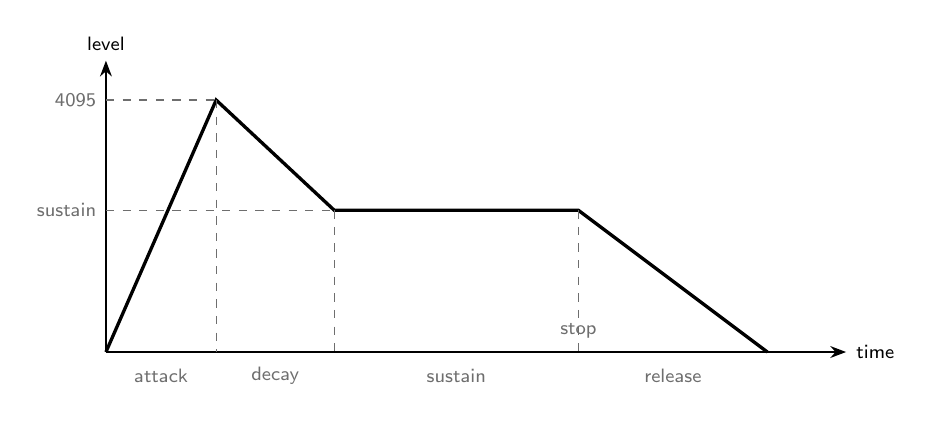
\begin{tikzpicture}[
			scale=1.0,
			axis/.style={-{Stealth[length=2mm]}, thick},
			note/.style={font=\scriptsize, text=sircgray}
		]
		\draw[axis] (0,0) -- (9.4,0) node[right, font=\scriptsize] {time};
		\draw[axis] (0,0) -- (0,3.7) node[above, font=\scriptsize] {level};
		\draw[very thick] (0,0) -- (1.4,3.2) -- (2.9,1.8) -- (6.0,1.8) -- (8.4,0);
		\draw[dashed, sircgray] (1.4,3.2) -- (1.4,0);
		\draw[dashed, sircgray] (2.9,1.8) -- (2.9,0);
		\draw[dashed, sircgray] (6.0,1.8) -- (6.0,0);
		\draw[dashed, sircgray] (0,3.2) -- (1.4,3.2);
		\draw[dashed, sircgray] (0,1.8) -- (2.9,1.8);
		\node[note, anchor=east] at (0,3.2) {4095};
		\node[note, anchor=east] at (0,1.8) {sustain};
		\node[note] at (0.7,-0.3) {attack};
		\node[note] at (2.15,-0.3) {decay};
		\node[note] at (4.45,-0.3) {sustain};
		\node[note] at (7.2,-0.3) {release};
		\node[note, anchor=south] at (6.0,0.05) {stop};
	\end{tikzpicture}
	\caption{The Envelope Phases}
	\label{fig:envelope}
\end{figure}

\section{Phases}
\label{sec:envelope-phases}

The envelope is updated once in every 64 output samples (an interval of about 2.0 ms, or 499.4 updates a second). At
each update it takes one step, as follows:

\begin{table}[H]
	\centering
	\begin{tabular}{lp{9cm}}
		\toprule
		\textbf{Phase} & \textbf{Behaviour at each update}                                                                                                                                             \\
		\midrule
		Attack         & The level rises by \texttt{ATTACK}. When it reaches 4095, it stops there and the phase becomes decay. \texttt{ATTACK} of 0 sets the level to 4095 at once                     \\
		Decay          & The level falls by \texttt{DECAY}, but not below the sustain level. When it reaches that level, the phase becomes sustain. \texttt{DECAY} of 0 sets the sustain level at once \\
		Sustain        & The level stays at the sustain level until the voice is stopped                                                                                                               \\
		Release        & The level falls by \texttt{RELEASE}. When it reaches 0 the envelope is inactive. \texttt{RELEASE} of 0 sets the level to 0 at once                                            \\
		Inactive       & The level is 0 and stays there. The voice is silent until a note starts                                                                                                       \\
		\bottomrule
	\end{tabular}
	\caption{Envelope Phases}
	\label{tab:envelope-phases}
\end{table}

\texttt{ATTACK}, \texttt{DECAY} and \texttt{RELEASE} are unsigned 8-bit steps in units of the 12-bit level. \texttt{SUSTAIN}
is an unsigned 8-bit level, converted to the 12-bit scale by repeating its top four bits below it: the 12-bit level is
$(\texttt{SUSTAIN} \ll 4) \mathbin{|} (\texttt{SUSTAIN} \gg 4)$. A \texttt{SUSTAIN} of 255 gives the full level, 4095, and 0
gives 0. When the sustain level is 0 the voice is silent once the decay ends, but it is still active as far as the rules of Section~\ref{sec:note-start} go: its envelope is in the sustain phase, not inactive.

A stop (Section~\ref{sec:reg-command}) puts the envelope in the release phase from whatever phase it is in. A stop on
an inactive envelope has no effect.

\section{Starting a Note}

A note that retriggers (Section~\ref{sec:note-start}) sets the level to 0 and the phase to attack, and takes the first
step at once, without waiting for the voice's next update. An \texttt{ATTACK} of 0 therefore reaches full level
immediately, and any other attack starts at its first step and not at 0. The voice's own update then continues at its
regular intervals.

A full-scale attack takes at most $(\lceil 4095 / \mathrm{step} \rceil - 1) \times 2.0$ ms after the note starts, since
the first regular update falls within one interval of the note. A full-scale decay or release takes at most $\lceil
	4095 / \mathrm{step} \rceil \times 2.0$ ms. Table~\ref{tab:envelope-times} gives $4095 / \mathrm{step}$ intervals of
2.0 ms.

\begin{table}[H]
	\centering
	\begin{tabular}{rr}
		\toprule
		\textbf{Step} & \textbf{Time for 4095 levels (about)} \\
		\midrule
		255           & 32 ms                                 \\
		128           & 64 ms                                 \\
		64            & 128 ms                                \\
		32            & 256 ms                                \\
		16            & 512 ms                                \\
		8             & 1.0 s                                 \\
		4             & 2.05 s                                \\
		2             & 4.1 s                                 \\
		1             & 8.2 s                                 \\
		\bottomrule
	\end{tabular}
	\caption{Envelope Step and Time}
	\label{tab:envelope-times}
\end{table}

A step of 1 is the slowest the envelope goes. A voice with an \texttt{ATTACK} of 1 is silent at first: with a step of 1
the level is 1, which is too small to produce any output after the volume is applied (Section~\ref{sec:voice-gain}),
and the voice becomes audible only after one or more updates, later for a lower volume.

\section{Update Timing}
\label{sec:envelope-timing}

The six voices do not update together. Their updates are spread evenly across the 64 output samples of each interval,
so that in any one output sample at most one voice updates, and the arithmetic of the updates does not pile up. Each
voice still updates once in 64 output samples; the stagger fixes only which sample of the interval it is. The
assignment is fixed and is the same after every reset: voice $n$ updates when the count of sample periods since reset,
modulo 64, equals $(64 - \lfloor 64n/6 \rfloor) \bmod 64$, which is 0, 54, 43, 32, 22 and 11 for voices 0 to 5.

An envelope update is visible to the mixer from the next output sample.

\section{Retriggering}

A note that retriggers a voice that is still active restarts its envelope at 0 (Section~\ref{sec:note-start}). The
sound of the old note is replaced at once by the start of the new one, with no crossfade. A new note, with a position
of 0, begins with the first byte of its sample at its new level, so the output moves in one sample from wherever the
old note was to the new note's first value. A tune that retriggers a voice while the previous note is still loud has a
step in the output at each note. Chapter~\ref{ch:programming} describes how an instrument is designed to avoid it.

\chapter{Mixer and Output}
\label{ch:mixer}

The mixer turns the sample bytes of the voices into the two output channels. For every output sample it scales each
voice by its envelope and volume, divides it between the channels by its pan, adds in the filter's output, applies the
master volume, and limits the result to 16 bits. All the arithmetic is integer. A right shift of a negative number
rounds towards minus infinity, and the accumulators and the output are limited and never wrap
(Section~\ref{sec:number-formats}).

\section{Voice Gain}
\label{sec:voice-gain}

The envelope and the voice's volume are combined into one gain, so that a voice needs one multiplication and not two.
The gain is a 12-bit number:

\begin{equation*}
	G = (\mathrm{level} \times \mathrm{volume}) \gg 8
\end{equation*}

\noindent where \emph{level} is the 12-bit envelope level and \emph{volume} is the volume in force, 0 to 255 (a volume that a
modulation voice steers is limited to this range). The sample byte is expanded to 16 bits by placing it in the high byte, and
the scaled sample is:

\begin{equation*}
	\mathrm{scaled} = ((\mathrm{sample} \ll 8) \times G) \gg 12
\end{equation*}

The largest gain is $(4095 \times 255) \gg 8 = 4079$, which is 0.9958 of unity, 0.036 dB below it. A voice at full
volume and full envelope therefore plays at 99.6\% of the sample's own level: a byte of $+127$ gives $+32{,}377$ and a
byte of $-128$ gives $-32{,}632$. The gain depends only on the envelope level and the volume in force, so it changes
only when one of them does.

\section{Panning and Mixing}
\label{sec:mixing}

A dry voice is divided between the two channels by its pan, an 8-bit number. The device finds the right channel's share
and takes the rest as the left:

\begin{equation*}
	\mathrm{right} = (\mathrm{scaled} \times \mathrm{pan}) \gg 8, \qquad \mathrm{left} = \mathrm{scaled} - \mathrm{right}
\end{equation*}

The two shares add up to the scaled sample, so the pan moves the sound between the channels and does not change its
total. A pan of 0 puts all of the voice in the left channel. A pan of 128 puts half in each, which is 6 dB below the
sample in each channel. A pan of 255 puts 255/256 in the right channel and the remaining 1/256 in the left, 48 dB
below, so the right-hand extreme is not quite a hard pan. The centre is 6 dB down in each channel by design: the pan
has no compensation, so a voice at centre is quieter in each channel than the same voice panned hard to one side.

Each channel has an accumulator, a signed 20-bit number. The shares of all the dry voices and of the filter are added
into the two accumulators. Six voices at full scale add to less than the range of the accumulator, but adding the
filter's output can take a sum past it, so each accumulator is limited to 20 bits after the filter's output is added.

\section{The Filter Bus}

A voice whose \texttt{FILTER\_EN} bit is set does not go to the accumulators. Its scaled sample is added to a single
sum, the filter input, which is a mono signal and is not panned. The filter's output is added to the accumulators with
its own volume and pan (Section~\ref{sec:filter-output}). A voice in modulation mode contributes to neither the
accumulators nor the filter input. Chapter~\ref{ch:filter} describes the filter.

\section{Master Volume and Limiting}
\label{sec:master-volume}

After the filter's output has been added, each accumulator is scaled by the master volume:

\begin{equation*}
	\mathrm{output} = (\mathrm{accumulator} \times \mathrm{master}) \gg 8
\end{equation*}

\noindent and limited to the signed 16-bit range, $-32{,}768$ to $+32{,}767$. A mix that is louder than that is
clipped, not wrapped. The master volume is the 8-bit value in \texttt{MASTER\_VOL}, adjusted by any modulation that
steers it (Chapter~\ref{ch:modulation}). At its reset value of 255, it passes 255/256 of the mix.

The limit is the only protection against a loud mix. There is no automatic gain control: six full-scale voices sent to
one channel clip.

\section{Output}

The two limited values are sent to the converter in the serial format of Chapter~\ref{ch:signal-timing}. While
\texttt{AUDIO\_EN} is 0 the device sends zero in both channels instead. The computation goes on as before, so the
voices are in the right place when the output is enabled.

A voice reads its sample byte in one sample period, the byte is scaled and mixed in the next, and the result is sent to
the converter in the one after that: three sample periods, about 94 $\mu$s, from a read to its effect at the converter
(Chapter~\ref{ch:timing}).

\chapter{Modulation}
\label{ch:modulation}

Any voice can be made a \emph{modulation source}. It then plays like any other voice, from an instrument, through an
envelope and a volume, but it makes no sound: its output steers one parameter of another voice or of the device. A
sample that is a slow sine wave gives vibrato, tremolo or a sweeping filter; a faster or more complex one gives
stranger effects. A modulation source takes a whole voice, so using one leaves five voices for sound.

\section{Modulation Sources}

A voice is a modulation source while its \texttt{MOD\_MODE} bit is 1 (Section~\ref{sec:reg-control}). Its scaled
sample, the same value a sounding voice would send to the mixer (Section~\ref{sec:voice-gain}), is the source value.
The device takes the high eight bits of it, a signed number from $-128$ to $+127$, and calls it $M$. The voice's volume
and envelope therefore set the depth of the modulation, and its sample sets the shape. A voice's \texttt{MOD\_ROUTE}
register says where its value goes; it is read only while \texttt{MOD\_MODE} is 1 (Section~\ref{sec:reg-mod-route}).

\section{Destinations}

\begin{table}[H]
	\centering
	\begin{tabular}{lllp{6.4cm}}
		\toprule
		\textbf{\texttt{DEST}} & \textbf{Destination} & \textbf{Voice field} & \textbf{Parameter steered}                \\
		\midrule
		0                      & Off                  & Ignored              & The voice is a source with no destination \\
		1                      & Pitch                & Used                 & The step of the destination voice         \\
		2                      & Volume               & Used                 & The volume of the destination voice       \\
		3                      & Pan                  & Used                 & The pan of the destination voice          \\
		4                      & Filter cutoff        & Ignored              & \texttt{FILTER\_CUTOFF}                   \\
		5                      & Master volume        & Ignored              & \texttt{MASTER\_VOL}                      \\
		6                      & Filter pan           & Ignored              & The pan byte of \texttt{FILTER\_VOL\_PAN} \\
		7                      & Reserved             & ---                  & Software must not use it                  \\
		\bottomrule
	\end{tabular}
	\caption{Modulation Destinations}
	\label{tab:mod-destinations}
\end{table}

The filter resonance cannot be modulated. A voice may modulate any voice, including itself.

\section{Scaling}
\label{sec:mod-scaling}

The change to the destination is:

\begin{equation*}
	\Delta = M \times 2^{\,\mathrm{SHIFT} + K}
\end{equation*}

\noindent where \texttt{SHIFT} is the signed field of \texttt{MOD\_ROUTE} ($-8$ to $+7$) and $K$ depends on the destination:
$K = 4$ for pitch and for filter cutoff, and $K = 0$ for volume, pan, master volume and filter pan. A negative exponent is an
arithmetic shift right. The \texttt{INV} bit negates $M$ first. The change is added to the value the destination
holds, and the sum is limited to the destination's range: 0 to 255 for volume, pan, master volume, filter cutoff and
filter pan, and 0 to the largest 16.16 value for the pitch step. The register itself is not changed: it keeps the value the
program wrote, and the sum is the value in force.

For volume and pan, a change of the value in force is a change in the same units as the register, so a shift of 0 with
a source of $+127$ moves the volume by 127 steps of the 256. For the cutoff the unit is a step of the cutoff register
(Chapter~\ref{ch:filter}). For pitch the unit is a raw unit of the 16.16 step.

\subsection{The Depth of Pitch Modulation}
\label{sec:mod-pitch-depth}

The pitch change is added to the step in raw units, so its size as a fraction of the pitch depends on the note. A
source of $+127$ with a shift of 0 adds $127 \ll 4 = 2032$ units. Table~\ref{tab:mod-pitch-depth} shows what that is,
in cents, for the 64-byte waveform of Table~\ref{tab:pitch-table}: a slow sine routed to a low note makes a wide swing,
and the same source routed to a high note a barely audible one. A program that wants an equal vibrato across the range
changes the shift as the octave changes.

\begin{table}[H]
	\centering
	\begin{tabular}{rr}
		\toprule
		\textbf{Note} & \textbf{Change for $M = +127$, shift 0 (cents)} \\
		\midrule
		0             & 773                                             \\
		24            & 228                                             \\
		48            & 59.9                                            \\
		72            & 15.2                                            \\
		96            & 3.8                                             \\
		119           & 1.0                                             \\
		\bottomrule
	\end{tabular}
	\caption{The Depth of Pitch Modulation (64-Byte Waveform)}
	\label{tab:mod-pitch-depth}
\end{table}

\section{Rules}

\begin{itemize}
	\item \textbf{One source for each destination.} At most one modulation source affects any destination. If several
	      voices route to the same destination, the one with the lowest voice number wins and the others have no effect. A
	      source with \texttt{DEST} of 0 does not take part.
	\item \textbf{One sample of delay.} A source's value is used by its destination from the next output sample after the
	      source's byte is read. Modulation can therefore be cascaded, and two voices can modulate each other, with no
	      loop that has to settle within one sample: the result is always determined.
	\item \textbf{The envelope comes first.} The envelope of the destination voice is applied before modulation. Modulating a
	      voice's volume never makes sound from a voice whose envelope is inactive, because the gain is the product of the
	      envelope and the volume (Section~\ref{sec:voice-gain}).
	\item \textbf{The programmed value stays.} A destination holds the value the program wrote. Switching the modulation
	      off, by clearing \texttt{MOD\_MODE} on the source or setting \texttt{DEST} to 0, returns the destination to it with
	      no further action.
\end{itemize}

\section{Making a Low-Frequency Oscillator}

A modulation voice is an ordinary voice, so its rate is set by its note and its instrument's pitch table. The lowest
note of a pitch table built for a waveform's real length is 27.5~Hz, which is too fast for vibrato. The program builds
the modulation instrument's pitch table for a cycle that is shorter than the waveform really is, so that its entries
are smaller: a 64-byte sine with a pitch table built as for a 12.8-byte cycle plays at one fifth of the usual rate,
5.5~Hz at note 0. Chapter~\ref{ch:programming} gives an example.

\chapter{The Shared Filter}
\label{ch:filter}

The device has one filter, shared by all the voices. It is a two-pole resonant filter of the state-variable kind, and
it can be a low-pass, a band-pass or a high-pass filter. Its input is the sum of the voices whose \texttt{FILTER\_EN}
bit is set; its output has its own volume and pan, and is mixed with the dry voices (Section~\ref{sec:filter-output}).
A voice that is filtered is not also heard dry.

\section{Operation}

The filter runs once for every output sample, all the time. It runs when no voice is routed to it, and while the output
is muted, so its state is always current. There is no register bit that turns it off. A program that does not want the
filter leaves its voices' \texttt{FILTER\_EN} bits clear.

The filter holds two state values, \emph{low} and \emph{band}. For each output sample, with the input \emph{in}, it
forms three results in this order:

\begin{align*}
	\mathrm{low}  & \leftarrow \mathrm{low} + f \times \mathrm{band}               \\
	\mathrm{high} & \leftarrow \mathrm{in} - \mathrm{low} - q \times \mathrm{band} \\
	\mathrm{band} & \leftarrow \mathrm{band} + f \times \mathrm{high}
\end{align*}

\noindent Each line uses the values the lines above it have just produced. The coefficient $f$ comes from the cutoff register
and $q$ from the resonance register (Sections~\ref{sec:filter-cutoff} and~\ref{sec:filter-resonance}). The output is
the new \emph{low}, \emph{band} or \emph{high}, as \texttt{FILTER\_CONFIG} selects: low-pass, band-pass or high-pass
(Table~\ref{tab:reg-filter}).

\begin{figure}[H]
	\centering
	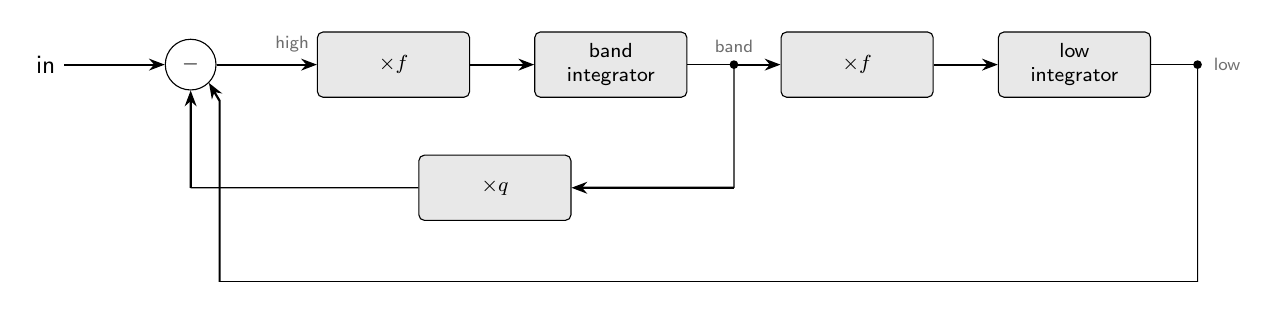
\begin{tikzpicture}[
			scale=0.92, transform shape,
			box/.style={draw, rounded corners=2pt, fill=sirclightgray, align=center, font=\footnotesize, minimum height=0.9cm, minimum width=2.1cm},
			sum/.style={draw, circle, fill=white, font=\footnotesize, inner sep=1pt, minimum size=0.7cm},
			flow/.style={-{Stealth[length=2mm]}, thick},
			note/.style={font=\scriptsize, text=sircgray}
		]
		\node (in) at (-1.2,0) {in};
		\node[sum] (s) at (0.8,0) {$-$};
		\node[box] (f1) at (3.6,0) {$\times f$};
		\node[box] (b) at (6.6,0) {band\\integrator};
		\node[box] (f2) at (10.0,0) {$\times f$};
		\node[box] (l) at (13.0,0) {low\\integrator};
		\node[box] (q) at (5.0,-1.7) {$\times q$};
		\coordinate (bandtap) at (8.3,0);
		\coordinate (lowtap) at (14.7,0);
		\draw[flow] (in) -- (s);
		\draw[flow] (s) -- (f1);
		\draw[flow] (f1) -- (b);
		\draw (b) -- (bandtap);
		\draw[flow] (bandtap) -- (f2);
		\draw[flow] (f2) -- (l);
		\draw (l) -- (lowtap);
		\fill (bandtap) circle (0.06);
		\fill (lowtap) circle (0.06);
		\draw (bandtap) -- (8.3,-1.7);
		\draw[flow] (8.3,-1.7) -- (q.east);
		\draw (q.west) -- (0.8,-1.7);
		\draw[flow] (0.8,-1.7) -- (s.south);
		\draw (lowtap) -- (14.7,-3.0);
		\draw (14.7,-3.0) -- (1.2,-3.0);
		\draw[flow] (1.2,-3.0) |- (1.2,-0.5) -- (s.south east);
		\node[note, above] at (2.2,0.05) {high};
		\node[note, above] at (8.3,0.05) {band};
		\node[note, right] at (14.8,0) {low};
	\end{tikzpicture}
	\caption{The Filter}
	\label{fig:filter}
\end{figure}

\section{Arithmetic}

The filter works on signed 24-bit numbers with four fraction bits: the input sum of the voices' scaled samples is
multiplied by 16 to enter them, and an output is divided by 16 (with the shift rounding towards minus infinity) and
limited to 20 bits to leave them. The coefficients $f$ and $q$ are 8-bit numbers divided by 256, so each multiplication
is a state value times an 8-bit coefficient shifted right by 8. The shift truncates: it rounds towards minus infinity.
The filter needs three multiplications for each output sample: $f \times \mathrm{band}$, $q \times \mathrm{band}$ and
$f \times \mathrm{high}$.

Every sum and every state is limited to the 24-bit range and never wraps around. A loud input or a high resonance can
therefore drive the filter into the limit, and the states are held at the limit of their range: they do not wrap, so
the filter stays bounded. The filter does not reduce its gain to avoid this, and it does not remove the small errors
its truncation leaves: after a loud sound ends, the output settles to within a few output units of zero (at worst about
5), and does not fall further, provided that the resonance is below 255.

\section{Cutoff}
\label{sec:filter-cutoff}

The cutoff register \texttt{FILTER\_CUTOFF} holds an unsigned 8-bit value $c$, and $f = c / 256$. The nominal cutoff
frequency of the filter, which is the frequency of its poles when the damping is zero and is close to it for light
damping, is

\begin{equation*}
	f_c = \frac{f_s}{\pi} \arcsin\!\left(\frac{f}{2}\right)
\end{equation*}

\noindent where $f_s$ is the output sample rate of 31,960.226~Hz. The largest value, 255, gives about 5.3~kHz. With heavy damping the peak of the band-pass response lies a little above the nominal frequency, about 6\% above at the lowest resonance. The frequency is nearly
proportional to the register: each step is about 20~Hz at the low end, and a little more higher up.

\begin{table}[H]
	\centering
	\begin{tabular}{rrr}
		\toprule
		\textbf{Register} & \textbf{Frequency (Hz)} & \textbf{Next step up (semitones)} \\
		\midrule
		1                 & 19.9                    & 12.0                              \\
		2                 & 39.7                    & 7.0                               \\
		4                 & 79.5                    & 3.9                               \\
		8                 & 159.0                   & 2.0                               \\
		16                & 318.0                   & 1.05                              \\
		32                & 636.2                   & 0.53                              \\
		64                & 1275.0                  & 0.27                              \\
		128               & 2570.6                  & 0.14                              \\
		192               & 3910.6                  & 0.09                              \\
		254               & 5280.9                  & 0.07                              \\
		255               & 5303.8                  & ---                               \\
		\bottomrule
	\end{tabular}
	\caption{Nominal Filter Cutoff Frequencies}
	\label{tab:filter-cutoff}
\end{table}

Because the register is linear in frequency, the musical size of a step falls as the cutoff rises: the first step is an
octave and a step at 2.5~kHz is about a seventh of a semitone. A slow sweep through the low end is therefore heard as
steps.

A cutoff register value of 0 makes $f$ zero, and then neither of the two lines that change the state of the filter does
anything: \emph{low} and \emph{band} hold their last values. The low-pass output is a constant, and the high-pass
output is the input less that constant and the damping term. The filter resumes from the held state when the cutoff is
raised, with no step. A program that wants the filter silent sets the volume byte of \texttt{FILTER\_VOL\_PAN} to 0, or
clears \texttt{FILTER\_EN} on its voices.

\section{Resonance}
\label{sec:filter-resonance}

The resonance register \texttt{FILTER\_RESONANCE} holds an unsigned 8-bit value $R$. It sets the damping of the filter,
$q = d / 256$, where for $R$ from 0 to 254

\begin{equation*}
	d = 16 + \left\lfloor \frac{3 (255 - R)}{4} \right\rfloor
\end{equation*}

\noindent and for $R = 255$ the damping is zero. A smaller damping gives a sharper and taller peak at the pole frequency.

\begin{table}[H]
	\centering
	\begin{tabular}{rrrr}
		\toprule
		\textbf{Resonance} & \textbf{$d$ ($q \times 256$)} & \textbf{$Q = 1/q$} & \textbf{Band-pass peak (dB)} \\
		\midrule
		0                  & 207                           & 1.2                & 1.9                          \\
		64                 & 159                           & 1.6                & 4.2                          \\
		128                & 111                           & 2.3                & 7.3                          \\
		192                & 63                            & 4.1                & 12.2                         \\
		224                & 39                            & 6.6                & 16.4                         \\
		240                & 27                            & 9.5                & 19.6                         \\
		250                & 19                            & 13.5               & 22.7                         \\
		254                & 16                            & 16.0               & 24.2                         \\
		255                & 0                             & unbounded          & ---                          \\
		\bottomrule
	\end{tabular}
	\caption{Filter Resonance (Cutoff Register 64)}
	\label{tab:filter-resonance}
\end{table}

A resonance of 255 is a special value: the damping is zero, so the filter does not lose energy. Once an input or a
nonzero state sets it going, it oscillates at the pole frequency with a constant amplitude, and that amplitude is held
until the state is disturbed again. A filter whose states are zero and whose input is zero stays silent. Values near
255 are very resonant but do damp.

\section{Filter Output}
\label{sec:filter-output}

The selected output, divided by 16 and limited to 20 bits, is scaled by the filter volume, the high byte of
\texttt{FILTER\_VOL\_PAN}, and divided between the channels by the filter pan, its low byte, as a voice is
(Sections~\ref{sec:voice-gain} and~\ref{sec:mixing}). The two shares are added to the accumulators with the dry voices.
A modulation source can steer the cutoff and the filter pan (Chapter~\ref{ch:modulation}). The resonance and the volume
cannot be steered.

At reset the filter's state is zero (Section~\ref{sec:reset}).

\chapter{The Sequencers}
\label{ch:sequencer}

Each voice has a sequencer that can play a tune from instructions in audio memory with no help from the CPU. The six
sequencers are independent: each has a program counter of its own, and each voice can run a different sequence. They
share one instruction decoder and one tick, so they keep time together.

\section{Operation}

A sequencer is enabled by its voice's \texttt{SEQ\_EN} bit. It starts at the window address its \texttt{SEQ\_PC}
register holds (Section~\ref{sec:seq-restart}) and runs one instruction at a time, each a single 16-bit word.

The tick is the sequencers' clock. \texttt{SEQ\_PERIOD} gives its period in output samples, from 1 to 65,535; a value
of 0 stops the ticks, and then no sequencer advances. On each tick every running sequencer executes instructions, in
program order, until it reaches a \texttt{WAIT}, finishes, or has executed eight instructions. Executing an instruction
can take several output samples, because reading it and, for a note, the instrument and pitch table take reads of audio
memory (Chapter~\ref{ch:timing}); the order of a voice's instructions is always preserved.

A sequencer keeps its program counter, a \texttt{WAIT} counter, an 8-bit \texttt{END} counter and a flag that says it
has finished.

\section{Instruction Set}
\label{sec:seq-instructions}

Every instruction is one 16-bit word. Bits 15--13 are the opcode and bits 12--0 are the operand.

\begin{figure}[H]
	\centering
	\begin{bytefield}[bitwidth=2em]{16}
		\bitheader{0-15} \\
		\bitbox{3}{OP} &
		\bitbox{13}{Operand}
	\end{bytefield}
	\caption{Sequencer Instruction Format}
	\label{fig:seq-format}
\end{figure}

\begin{table}[H]
	\centering
	\begin{tabular}{lllp{5.1cm}}
		\toprule
		\textbf{Opcode} & \textbf{Instruction} & \textbf{Operand}                       & \textbf{Effect}                                               \\
		\midrule
		000             & \texttt{NOTE}        & Bits 6--0: note, 0--119                & Starts a note, or glides to it (Section~\ref{sec:note-start}) \\
		001             & \texttt{STOP}        & Unused                                 & Starts the envelope release                                   \\
		010             & \texttt{WAIT}        & Bits 12--0: ticks, 1--8191             & Waits that number of ticks                                    \\
		011             & \texttt{INST}        & Bits 7--0: instrument number           & Selects the instrument for the next note                      \\
		100             & \texttt{FINE}        & Bits 12--0: signed                     & Sets the fine pitch adjustment                                \\
		101             & \texttt{GOTO}        & Bits 12--0: signed, $-4096$ to $+4095$ & Jumps by that many instruction words                          \\
		110             & \texttt{END}         & Bits 7--0: count, 0--255               & Ends the sequence, now or after a count                       \\
		111             & ---                  & ---                                    & Reserved                                                      \\
		\bottomrule
	\end{tabular}
	\caption{Sequencer Instructions}
	\label{tab:seq-instructions}
\end{table}

Operand bits that an instruction does not use are reserved. A reserved opcode is ignored: it does nothing but use one
of the eight instructions of the tick. A \texttt{NOTE} with a number above 119 is ignored in the same way. Software
must not rely on either.

\begin{description}
	\item[\texttt{NOTE}] Starts the note given, on the instrument in \texttt{INSTR}. The voice retriggers or glides as
	      Section~\ref{sec:note-start} describes, and the sequencer carries on with the instruction after \texttt{NOTE}
	      when the note has been applied.
	\item[\texttt{STOP}] Starts the release of the voice's envelope.
	\item[\texttt{WAIT}] Sets the voice's \texttt{WAIT} counter to the operand and ends the voice's work for the tick. At
	      each later tick the counter is decremented, and when it reaches 0 the voice carries on, in that same tick, with
	      the instruction after the \texttt{WAIT}. A \texttt{WAIT} of 1 therefore carries on at the next tick, and the notes of
	      \texttt{NOTE}, \texttt{WAIT 1}, \texttt{NOTE} are one tick apart. A \texttt{WAIT} of 0 delays nothing and is not
	      the same as 1: software must not use it.
	\item[\texttt{INST}] Writes the operand to the voice's \texttt{INSTR} register.
	\item[\texttt{FINE}] Writes the signed operand to the voice's \texttt{FINE} register.
	\item[\texttt{GOTO}] Adds the signed operand to the address of the instruction after the \texttt{GOTO}, in instruction
	      words. A displacement of $-1$ jumps back to the \texttt{GOTO} itself; $-2$ jumps to the instruction before it. The
	      address wraps within the window.
	\item[\texttt{END}] Ends the sequence now or after a count (Section~\ref{sec:seq-end}).
\end{description}

\subsection{Counted END}
\label{sec:seq-end}

An \texttt{END} of 0 ends the sequence at once. An \texttt{END} of $N$, for $N$ from 1 to 255, adds 1 to the voice's
\texttt{END} counter (which stops at 255), and ends the sequence if the counter is then $N$ or more; otherwise the
sequencer carries on with the instruction after the \texttt{END}. A sequence that loops can therefore play a section a
number of times.

All the \texttt{END} instructions of a voice share one counter. \texttt{GOTO} does not reset it, there are no nested
counts, and only a write to \texttt{SEQ\_PC} clears it (Section~\ref{sec:seq-restart}).

When a sequence ends, the voice's flag in \texttt{SEQ\_DONE} is set, exactly once, and the sequencer stops. The voice
carries on playing its sample under its envelope. The sequencer stays stopped until \texttt{SEQ\_PC} is written.

\subsection{An Example}

Table~\ref{tab:seq-example} is a sequence that plays two notes, each held for ten ticks, and repeats five times. The
instrument is set by the program that starts it, or by an \texttt{INST} before the first note.

\begin{table}[H]
	\centering
	\begin{tabular}{rlll}
		\toprule
		\textbf{Word} & \textbf{Instruction} & \textbf{Encoding} & \textbf{Comment}                                       \\
		\midrule
		0             & \texttt{NOTE 48}     & \texttt{0x0030}   & A4 with the pitch table of Table~\ref{tab:pitch-table} \\
		1             & \texttt{WAIT 10}     & \texttt{0x400A}   &                                                        \\
		2             & \texttt{NOTE 50}     & \texttt{0x0032}   & B4                                                     \\
		3             & \texttt{WAIT 10}     & \texttt{0x400A}   &                                                        \\
		4             & \texttt{END 5}       & \texttt{0xC005}   & Ends on the fifth pass                                 \\
		5             & \texttt{GOTO} $-6$   & \texttt{0xBFFA}   & Back to word 0                                         \\
		\bottomrule
	\end{tabular}
	\caption{An Example Sequence}
	\label{tab:seq-example}
\end{table}

The sequence plays its two notes five times and sets its \texttt{SEQ\_DONE} flag. It is then halted until
\texttt{SEQ\_PC} is written again.

\section{Restarting a Sequence}
\label{sec:seq-restart}

A write to \texttt{SEQ\_PC} restarts the voice's sequence at the address written. It clears the voice's \texttt{WAIT}
counter and \texttt{END} counter and its \texttt{SEQ\_DONE} flag, and starts the sequencer if it had finished. Any
instruction fetch or note load that was in progress is abandoned; what had already been applied, such as a note that
has started to sound, stays. The sequencer then runs on the next tick if \texttt{SEQ\_EN} is 1, and not before. A voice
whose \texttt{SEQ\_EN} is 0 does not run a sequence, and writing \texttt{SEQ\_PC} only sets up its counter.

\section{Completion Interrupt}
\label{sec:interrupts}

The device has one interrupt, \activelow{IRQ3}, for the end of a sequence. The signal is asserted whenever the logical
AND of any bit of \texttt{SEQ\_DONE} and the same bit of \texttt{SEQ\_INT\_EN} is 1 (Section~\ref{sec:reg-sequencer}).
It is level-sensitive: it is released when the program has cleared the enabled flags, by writing 1s to
\texttt{SEQ\_DONE}, or has disabled their interrupts. A sequence that ended while its interrupt was disabled asserts
the signal when the interrupt is enabled afterwards. The \texttt{SEQ\_IRQ} bit of \texttt{STATUS} follows the signal. A
handler that does not clear the flag is entered again as soon as it returns. Writing \texttt{SEQ\_PC} also clears the
voice's flag.

\section{Deadlines}
\label{sec:seq-deadlines}

The work that a tick starts must be finished before the next tick. A voice that has not finished its work when the next
tick comes is not started again: it misses that tick, its \texttt{WAIT} counter is not decremented for it, and the
\texttt{MEM\_OVERRUN} bit of \texttt{STATUS} is set. The rest of its work then completes as before, so the music slows
by the ticks that were missed. A program avoids the condition by keeping the work in each tick small, and by choosing a
tick that is not too short (Section~\ref{sec:deadlines}).

\section{Direct Control and Sound Effects}
\label{sec:direct-control}

The device has no separate engine for sound effects. A voice with \texttt{SEQ\_EN} clear is controlled by the CPU: it
writes \texttt{INSTR} and \texttt{FINE}, then \texttt{COMMAND} to start or stop a note. The other voice registers,
volume, pan, portamento, routing and modulation, can be written in either mode. The CPU can take a voice from the
sequencer by clearing \texttt{SEQ\_EN}, play an effect, and give it back by setting \texttt{SEQ\_EN} and writing
\texttt{SEQ\_PC}: setting \texttt{SEQ\_EN} alone does not restart the sequence (Section~\ref{sec:reg-control}).

\chapter{Timing}
\label{ch:timing}

This chapter gives the timing inside the device: the clock, the sample period, the pattern in which the audio memory is
shared, and the deadlines that the pattern sets. Chapter~\ref{ch:signal-timing} gives the timing of the pins.

\section{Clocks and Periods}

The system oscillator of an NTSC system runs at 21,477,272 Hz. The device is clocked at half that rate by
\texttt{CLKI}, 10,738,636 Hz, a period of 93.1 ns. Everything the device does is a whole number of \texttt{CLKI}
cycles. The system oscillator of a PAL system runs at 21,281,370 Hz, so its \texttt{CLKI} is 10,640,685 Hz, a period of
94.0 ns. The figures in Table~\ref{tab:periods} are for an NTSC system; Section~\ref{sec:clock-rate} gives the PAL
values.

\begin{table}[H]
	\centering
	\begin{tabular}{p{3.6cm}p{3.6cm}p{5.2cm}}
		\toprule
		\textbf{Quantity}              & \textbf{Value}                               & \textbf{Derivation}                                  \\
		\midrule
		\texttt{CLKI} period           & 93.1 ns                                      & 2 oscillator periods                                 \\
		Output sample period           & 336 cycles, 31.29 $\mu$s                     & 672 oscillator periods                               \\
		Output sample rate             & 31,960.226 Hz                                & \texttt{CLKI} / 336                                  \\
		Envelope update interval       & 64 samples, 2.002 ms                         & 21,504 cycles; 499.4 updates a second for each voice \\
		Serial bit clock \texttt{BCLK} & 10 and 11 cycles alternately, 1.023 MHz mean & 32 bits in a sample period; 16 in each slot          \\
		Memory transaction             & 2 cycles, 186 ns                             & One read or one write                                \\
		Sequencer tick                 & \texttt{SEQ\_PERIOD} samples                 & Chosen by the program                                \\
		\bottomrule
	\end{tabular}
	\caption{Clocks and Periods}
	\label{tab:periods}
\end{table}

The output sample period is the device's hard deadline. Each period the device must read the next sample byte of every
voice that is playing a sample and produce the next stereo output sample. The sequencers have a softer one: their work
may run over several sample periods, but it must finish before the next tick (Section~\ref{sec:seq-deadlines}). The
sample generator and the memory schedule run continuously, whether the output is muted or not.

\section{Clock Rate}
\label{sec:clock-rate}

The device has one clock, \texttt{CLKI}, and every interval it measures is a count of \texttt{CLKI} cycles. It works at
any steady clock from 9.0 to 12.0~MHz. The system supplies the clock: a system whose oscillator differs from the one in
Table~\ref{tab:periods} divides it to a frequency in this range.

\begin{table}[H]
	\centering
	\begin{tabular}{lrrr}
		\toprule
		\textbf{Quantity}                     & \textbf{Minimum} & \textbf{Nominal} & \textbf{Maximum} \\
		\midrule
		\texttt{CLKI} frequency               & 9.000 MHz        & 10.738636 MHz    & 12.000 MHz       \\
		\texttt{CLKI} period                  & 111.1 ns         & 93.1 ns          & 83.3 ns          \\
		Output sample rate                    & 26,786 Hz        & 31,960 Hz        & 35,714 Hz        \\
		Envelope update interval              & 2.389 ms         & 2.002 ms         & 1.792 ms         \\
		Serial bit clock \texttt{BCLK} (mean) & 0.857 MHz        & 1.023 MHz        & 1.143 MHz        \\
		Memory transaction (2 cycles)         & 222.2 ns         & 186.2 ns         & 166.7 ns         \\
		Pitch against the nominal clock       & $-306$ cents     & 0                & $+192$ cents     \\
		\bottomrule
	\end{tabular}
	\caption{Clock Rate Range}
	\label{tab:clock-range}
\end{table}

Changing the clock changes every time the device keeps, in proportion: the sample rate, the envelope update interval,
the length of a tick of \texttt{SEQ\_PERIOD} samples, the rate of the serial output, and the pitch of every note. It
changes no behaviour measured in cycles or samples. The memory schedule, the number of instructions a sequence may run
in a tick, and the latency of a window access in cycles are the same at any clock in the range.

\subsection{Pitch at a Different Clock}

A pitch table (Section~\ref{sec:pitch-table}) gives each note a step in sample bytes per output sample, so the pitch
that a step produces is proportional to the sample rate, $\mathrm{CLKI} / 336$. A program that wants a note at an exact
frequency builds its tables for the clock of the system it runs on. A program that uses tables built for the nominal
clock plays every note sharp or flat in the ratio of the two clocks, by the amount in the last row of
Table~\ref{tab:clock-range} at the ends of the range. The tempo of a sequence changes by the same ratio. A program that
must keep time with the display, for example, counts display frames and not sequencer ticks.

In a PAL system the sample rate is 31,668.7~Hz, the ratio of the two clocks is 0.9909, and every note is 15.9 cents
flat of the same note in an NTSC system. Every time the device keeps, from an envelope update of 2.021~ms to a tick, is
0.9\% longer.

\subsection{What the Rest of the System Must Provide}

The device does not read or report its clock. The parts around it must keep up with the highest clock the system will
use:

\begin{itemize}
	\item \textbf{Audio memory.} The memory must complete an access within two \texttt{CLKI} cycles, less the set-up and
	      hold times of the interface, which are not yet specified. At the maximum clock this is 166.7 ns.
	\item \textbf{Converter.} The converter must accept a bit clock of 10 and 11 \texttt{CLKI} cycles alternately and a word rate of
	      \texttt{CLKI}/336 (Section~\ref{sec:converter-interface}).
	\item \textbf{Output filter.} The filter that follows the converter removes the images of the signal around the
	      sample rate. It is designed for the sample rate of the system, and must pass the highest frequency to be played
	      and stop the lowest image.
\end{itemize}

The clock must be continuous and steady while the device is running. The behaviour of the device when the clock
frequency changes while it runs is not yet specified.

\section{The Audio Memory Schedule}
\label{sec:memory-schedule}

The audio memory has two users, the sound processor and the CPU's window, and the device never makes them compete. It
divides time into a fixed pattern of eight cycles, made of four slots of two cycles. One slot belongs to the sound
processor and three to the CPU:

\begin{table}[H]
	\centering
	\begin{tabular}{lll}
		\toprule
		\textbf{Slot} & \textbf{Cycles of the pattern} & \textbf{Owner}  \\
		\midrule
		0             & 0--1                           & Sound processor \\
		1             & 2--3                           & CPU window      \\
		2             & 4--5                           & CPU window      \\
		3             & 6--7                           & CPU window      \\
		\bottomrule
	\end{tabular}
	\caption{The Audio Memory Schedule}
	\label{tab:memory-schedule}
\end{table}

\begin{figure}[H]
	\centering
	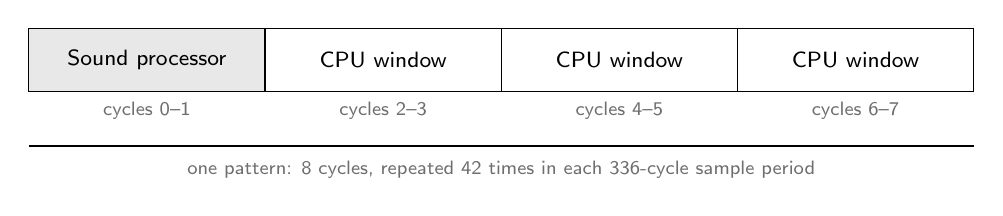
\begin{tikzpicture}[
			slot/.style={draw, minimum height=0.8cm, minimum width=3.0cm, align=center, font=\footnotesize},
			note/.style={font=\scriptsize, text=sircgray}
		]
		\foreach \i/\label/\fillc in {0/Sound processor/sirclightgray, 1/CPU window/white, 2/CPU window/white, 3/CPU window/white} {
				\node[slot, fill=\fillc] at (\i*3.0+1.5,0) {\label};
				\node[note] at (\i*3.0+1.5,-0.65) {cycles \number\numexpr\i*2\relax--\number\numexpr\i*2+1\relax};
			}
		\draw[thick] (0,-1.1) -- (12.0,-1.1);
		\node[note] at (6.0,-1.4) {one pattern: 8 cycles, repeated 42 times in each 336-cycle sample period};
	\end{tikzpicture}
	\caption{One Pattern of the Memory Schedule}
	\label{fig:memory-schedule}
\end{figure}

A sample period of 336 cycles holds exactly 42 patterns, so it holds 42 sound-processor slots and 126 CPU slots, in the
same places in every sample period. No slot can be borrowed: the sound processor never takes a CPU slot, and the CPU
never takes a sound-processor slot, whether or not the owner has anything to do. A slot that its owner does not use is
left idle.

\subsection{CPU Slots}
\label{sec:cpu-slots}

A CPU access to the audio memory is held until the next CPU slot, takes two cycles, and is then acknowledged. It is
acknowledged in the second to the fifth cycle of the access, counting the cycle in which the access is made as the
first (Table~\ref{tab:cpu-latency}). The time does not depend on the voices, the sequencers or the filter. The CPU
window can move 126 words, 252 bytes, in each sample period, which is 4.03 million words a second. How fast a block
move actually runs depends also on the bus cycle of the CPU (\hwmanual{}). Register accesses use no slot and are never
delayed.

\begin{table}[H]
	\centering
	\begin{tabular}{p{5.2cm}cccccccc}
		\toprule
		\textbf{Access made in cycle}  & 0 & 1 & 2 & 3 & 4 & 5 & 6 & 7 \\
		\midrule
		\textbf{Acknowledged in cycle} & 4 & 3 & 2 & 3 & 2 & 3 & 2 & 5 \\
		\bottomrule
	\end{tabular}
	\caption{CPU Window Access Time (Cycles of the Eight-Cycle Pattern)}
	\label{tab:cpu-latency}
\end{table}

An access made in the first cycle of a CPU slot (cycles 2, 4 and 6) is the quickest. The slowest is one made in the
last cycle of the pattern, which has to wait for the first CPU slot of the next.

\subsection{Sound Processor Slots}
\label{sec:spu-slots}

The sound processor uses its 42 slots for each sample period as follows, in this order of priority:

\begin{enumerate}
	\item \textbf{Sample reads.} A voice that is playing needs one word at most in each sample period, since it uses one
	      byte. Six voices need six slots at most. The reads are made first in the period.
	\item \textbf{Sequencer reads.} The slots that remain, at least 36 in each sample period, serve the sequencers. An
	      instruction takes one read. A note that loads a new instrument takes up to nine more: seven for the instrument
	      record and two for the pitch table entry; a note on the instrument the voice already has takes two.
\end{enumerate}

The voices share the sequencer slots in turn, so no voice waits for all of another's.

\section{Deadlines and Overrun}
\label{sec:deadlines}

The device sets the \texttt{MEM\_OVERRUN} bit of \texttt{STATUS} when it misses a deadline:

\begin{itemize}
	\item A sample read is not complete when the sample period ends. The slots set aside for sample reads make this impossible
	      while the device is working within its limits.
	\item The sequencer work started by a tick is not complete when the next tick comes (Section~\ref{sec:seq-deadlines}).
\end{itemize}

Work that takes longer than one sample period is not a missed deadline in itself. The bit is held until the program
clears it through \texttt{STATUSCLR}. An overrun never takes a slot from the CPU, and it never stops the voices: sample
reads go on, and a voice whose tick was missed is simply started again at the next one.

\subsection{Choosing a Tick}
\label{sec:choosing-tick}

How short a tick can be depends on how much the sequences do in each. A voice executes at most eight instructions in a
tick, and each instruction is one read; a note also reads its instrument record when the instrument has changed (seven
reads) and its pitch table entry (two). Six voices share at least 36 sequencer slots in each sample period, so the
number of reads in a tick, divided by 36, gives the shortest tick in sample periods that cannot overrun.
Table~\ref{tab:tick-limits} works out three cases.

\begin{table}[H]
	\centering
	\small
	\begin{tabular}{p{7.4cm}rrr}
		\toprule
		\textbf{Case, for each voice in one tick}                                                   & \textbf{Reads} & \textbf{Six voices} & \textbf{Periods at least} \\
		\midrule
		Worst: eight instructions, four of them notes on a different instrument                     & 44             & 264                 & 8                         \\
		A note on a new instrument and three other instructions                                     & 13             & 78                  & 3                         \\
		Notes on the instrument already loaded, with \texttt{INST}, \texttt{FINE} and \texttt{WAIT} & 6              & 36                  & 1                         \\
		\bottomrule
	\end{tabular}
	\caption{Reads in a Tick}
	\label{tab:tick-limits}
\end{table}

These are bounds. A sequence that waits between notes does less in most ticks, so a tick can be shorter than the table
says. A tick of 50 to 200 a second leaves nearly all of the slots idle.

\section{Latency}

A voice's sample byte is read during one sample period, scaled and mixed during the next, and sent to the converter
during the one after. The delay from a read to its sound at the output is three sample periods, 94 $\mu$s. A note takes
effect after the device has read its instrument record and pitch entry, which takes a sample period or two, and its
first sample byte then goes through the three periods above, so a note sounds within about five sample periods, 0.16
ms, of the sequencer reaching it. A note on a voice that already has its instrument is sooner. A write to a voice
register, such as volume, is seen from the next sample period.

\chapter{Signal Timing}
\label{ch:signal-timing}

This chapter gives the timing of the pins of the device (Chapter~\ref{ch:package}): the bus cycles in which the CPU
reads and writes it, the interrupt output, reset, and the serial output. Chapter~\ref{ch:timing} gives the timing
inside the device, in the same units.

\section{Reading the Figures}

The figures follow the conventions of the bus timing diagrams of the \hwmanual{}. Each labeled interval is one
\texttt{CLKI} cycle, seen between rising edges. Waveform rows show physical levels: for an active-low signal,
\texttt{L} means asserted. Bands show a value; an empty band carries no defined value, and a three-state signal that is
not driven is drawn as a flat line at mid-level. Electrical delays are not specified, so the figures show logical
timing only.

\section{Bus Cycles}
\label{sec:signal-bus}

The device answers every cycle in which \activelow{CS} and \activelow{BAS} are both asserted. How soon it asserts
\activelow{BACK} depends on the address: a register is answered in the cycle itself, and a word of the audio memory
window when the device has made the access.

\subsection{Register Accesses}

A register read or write is completed in the cycle in which it is made: \activelow{BACK} is asserted from the start of
the cycle, so the CPU accepts the cycle at the next rising edge and does not wait. On a write the register holds the
new value from that edge, and a read in the next cycle returns it. A write to a reserved offset is acknowledged in the
same way and changes nothing.

\begin{figure}[H]
	\centering
	\small
	\begin{tikztimingtable}[sirc timing diagram]
		CLKI             & L 2{0.5H 0.5L}              \\
		Phase            & D{access} D{next} D{}       \\
		\activelow{CS}   & L H H                       \\
		\activelow{BAS}  & L H H                       \\
		BRW              & L H H                       \\
		A0--A15          & D{offset} D{} D{}           \\
		D0--D15          & D{data} Z Z                 \\
		\activelow{BACK} & L H H                       \\
		Register         & D{old} 2D{new}              \\
	\end{tikztimingtable}
	\caption{Register Write Cycle}
	\label{fig:signal-write}
\end{figure}

On a read the device drives D0--D15 with the register's value from the start of the cycle to its end, and releases the
bus after it. A read changes nothing in the device.

\subsection{Audio Memory Window Accesses}

An access to the window waits for a CPU slot of the memory schedule (Section~\ref{sec:cpu-slots}). The CPU holds its
signals and the device holds \activelow{BACK} deasserted until the access is made, then asserts \activelow{BACK} for
the cycle in which a read puts its data on D0--D15, or a write takes its data. A window access is acknowledged in the
second to fifth cycle of the access, whatever the voices are doing (Section~\ref{sec:cpu-slots}).
Figure~\ref{fig:signal-window-read} shows a read of the slowest case, five cycles.

\begin{figure}[H]
	\centering
	\small
	\begin{tikztimingtable}[sirc timing diagram]
		CLKI             & L 5{0.5H 0.5L}                    \\
		Phase            & D{access} 3D{wait} D{done} D{}    \\
		\activelow{CS}   & 5L H                              \\
		\activelow{BAS}  & 5L H                              \\
		BRW              & 6H                                \\
		A0--A15          & 5D{offset} D{}                    \\
		D0--D15          & 4Z D{data} Z                      \\
		\activelow{BACK} & 4H L H                            \\
	\end{tikztimingtable}
	\caption{Audio Memory Window Read Cycle with Waits}
	\label{fig:signal-window-read}
\end{figure}

\section{Interrupt Output}

\activelow{IRQ3} is asserted while any \texttt{SEQ\_DONE} flag is set and its interrupt is enabled, and released when no
such flag remains (Section~\ref{sec:interrupts}). It is level-sensitive; no edge is produced. Its delay from the change
of the flags is not yet specified.

\section{Reset}

While \activelow{RST} is asserted the device holds the reset state of Section~\ref{sec:reset}. The converter output is
digital zero from reset until the program sets \texttt{AUDIO\_EN}. No interrupt is raised by reset. The minimum width
of the reset pulse is not yet specified.

\section{Serial Output}
\label{sec:serial-output}

The device sends one stereo sample every 336 \texttt{CLKI} cycles. The frame has 32 bit clocks, \texttt{BCLK}, in two
slots of 16, one for each channel. The periods of \texttt{BCLK} are 10 and 11 \texttt{CLKI} cycles alternately, the
first of the frame being 10, so the frame is $16 \times 10 + 16 \times 11 = 336$ cycles. The pattern is the same in
every frame, so every edge of \texttt{BCLK} falls at the same cycle of the frame each time. \texttt{WS} is low during
the left slot and high during the right. The duty cycle of \texttt{BCLK} is not yet specified.

\begin{table}[H]
	\centering
	\begin{tabular}{llp{6.4cm}}
		\toprule
		\textbf{\texttt{BCLK} periods of the frame} & \textbf{\texttt{WS}} & \textbf{\texttt{SD}}                          \\
		\midrule
		0                                           & Low                  & Bit 0 of the right word of the previous frame \\
		1--15                                       & Low                  & Bits 15 to 1 of the left word                 \\
		16                                          & High                 & Bit 0 of the left word                        \\
		17--31                                      & High                 & Bits 15 to 1 of the right word                \\
		\bottomrule
	\end{tabular}
	\caption{Serial Frame Layout}
	\label{tab:serial-frame}
\end{table}

The format is that of a standard two-channel serial audio interface. \texttt{WS} changes one bit clock before the most
significant bit of the word it announces, so the slot is as wide as the word and the last bit of each word is sent in
the first period of the next slot, after \texttt{WS} has changed. The 16 data bits are the output sample as a signed
two's-complement number, most significant first. A slot carries nothing else. The alignment of the edges of \texttt{WS}
and \texttt{SD} to \texttt{BCLK}, their set-up and hold times, and the \texttt{SCK} frequency and phase, are not yet
specified.

\chapter{Programming the Device}
\label{ch:programming}

This chapter collects what a program does in what order. It adds no new behaviour of the device; each rule is stated
where the feature is described, and the sections of the earlier chapters are cited.

\section{Starting Up}
\label{sec:startup}

At reset the output is silent (\texttt{AUDIO\_EN} is 0), the registers listed in Table~\ref{tab:reset} are set, and the
audio memory is undefined. A program starts the device in this order:

\begin{enumerate}
	\item Write the audio memory through the window (Chapter~\ref{ch:memory-map}): the instrument table, the pitch tables, the
	      sequences and the sample data. A voice that plays a word the program has not written plays noise.
	\item Write \texttt{INSTR\_BASE} with the window address of the instrument table.
	\item Write \texttt{MASTER\_VOL}, and the filter registers if any voice is filtered (Section~\ref{sec:reg-filter}).
	\item For each voice, write \texttt{CONTROL}, \texttt{VOLUME\_PAN}, \texttt{PORTA\_RATE} and, for a modulation voice,
	      \texttt{MOD\_ROUTE}. A voice's reset volume is 0, so it is silent until its volume is set.
	\item If a handler will serve the completion interrupt, install it, then write \texttt{SEQ\_INT\_EN}
	      (Section~\ref{sec:interrupts}).
	\item Write \texttt{CONFIG} to set \texttt{AUDIO\_EN}.
	\item For each voice that runs a sequence, set \texttt{SEQ\_EN} in \texttt{CONTROL} and write \texttt{SEQ\_PC}. Write
	      \texttt{SEQ\_PERIOD} last: the sequences then all start on the first tick.
\end{enumerate}

\section{Playing a Note by Hand}

A voice with \texttt{SEQ\_EN} clear is played from the CPU. To start a note, write the instrument number to
\texttt{INSTR}, then write \texttt{COMMAND} with bit 15 set and the note number in bits 6--0. To release it, write
\texttt{COMMAND} with bit 15 clear. The note sounds a few sample periods after the write
(Section~\ref{sec:note-start}); the CPU is not told when. A sound effect is a voice borrowed in this way: clear its
\texttt{SEQ\_EN}, play the effect, and give the voice back with \texttt{SEQ\_EN} and a write to \texttt{SEQ\_PC},
having saved \texttt{SEQ\_PC} beforehand (Section~\ref{sec:direct-control}).

\section{Building an Instrument}

\begin{itemize}
	\item \textbf{Waveform length.} The lookup does not interpolate, so a short waveform is noisier than a long one: the
	      error is about 24 dB below the signal for 64 bytes and 36 dB for 256, and it falls 6 dB with each doubling
	      (Section~\ref{sec:playing}). A waveform of 256 bytes or more is a good length for a clean tone. A single cycle in a loop
	      is cheap in memory, and can be played at any pitch below half the output rate.
	\item \textbf{Pitch table.} Build one for each distinct waveform length, from the formula of
	      Section~\ref{sec:pitch-table}. Instruments that use the same waveform can share a table.
	\item \textbf{Where the waveform starts.} A note starts at byte 0. A waveform that starts near zero, a sine or triangle
	      from its zero crossing for example, begins smoothly, and one that starts at a peak, the usual form of a sawtooth, does
	      not.
	\item \textbf{The envelope against retriggering.} A note on a sounding voice replaces it at once, with a step in the
	      output (Chapter~\ref{ch:envelope}). The step is small if the old note has died away. For notes that are played
	      one after another on one voice, choose a decay that reaches silence before the next note, or a gentle attack, or start the next note only after the envelope has become inactive. A voice with portamento enabled does not retrigger when the note is on
	      the same instrument and is still active.
	\item \textbf{Looping.} A loop shorter than the step is architecturally undefined (Section~\ref{sec:looping}). A
	      single-cycle waveform never meets it.
\end{itemize}

\section{Timing a Sequence}

A tick is the smallest time step of a sequence, and a \texttt{WAIT} of $n$ is $n$ ticks. A tick of 5 to 15
milliseconds, a \texttt{SEQ\_PERIOD} of 160 to 480 samples, gives fine control of timing, and a note is then held with
a \texttt{WAIT} of several ticks. Portamento and envelopes run on their own 2.0 ms clock and do not depend on the tick,
so the tick can be chosen for the music alone. A tick that is too short for the work in it overruns
(Section~\ref{sec:choosing-tick}).

\section{Vibrato and Other Effects}

Vibrato needs a modulation voice with a slow sine wave, routed to the pitch of the voice that plays the tune
(Chapter~\ref{ch:modulation}):

\begin{enumerate}
	\item Make an instrument with a sine of 64 bytes, looped, with an attack of 0 and a sustain of 255. Build its pitch table
	      with entries one fifth of those of Table~\ref{tab:pitch-table}, so that note 0 gives 5.5~Hz (the entry for note 0 is
	      722, \texttt{0x02D2}).
	\item Set the voice in modulation mode with a volume of 255, and write its \texttt{MOD\_ROUTE} with destination 1 (pitch),
	      the number of the voice to steer, and a shift of $-2$.
	\item Start note 0 on it.
\end{enumerate}

With a sine of amplitude 127 the pitch changes by at most $127 \times 4 = 508$ raw units, which for a 64-byte waveform
is a peak deviation of about 17 cents at G4 and 8.5 cents at G5, since pitch modulation is added in raw units
(Section~\ref{sec:mod-pitch-depth}). A greater shift deepens it. Tremolo routes to a voice's volume, a sweeping pan to
its pan, and a filter that wobbles to the cutoff.

A filter sweep is written by the program: change \texttt{FILTER\_CUTOFF} at a steady rate, for example once every few
milliseconds. A slow sweep through the lowest registers is heard in steps (Section~\ref{sec:filter-cutoff}).

\section{Programming Cautions}
\label{sec:cautions}

\begin{enumerate}
	\item \textbf{Audio memory.} The memory is undefined at reset. Write everything a voice or a sequence reads before it
	      starts (Section~\ref{sec:audio-memory}).
	\item \textbf{Instrument changes.} A voice reads its instrument record when the instrument changes, not on each note.
	      To change a record that a voice has loaded, change it, play a note on a different instrument, and then play a note on the changed one
	      (Section~\ref{sec:note-start}).
	\item \textbf{Retrigger steps.} A new note on an active voice makes a step in the output unless the old one has died
	      away (Chapter~\ref{ch:envelope}).
	\item \textbf{Fine pitch.} A raw unit of \texttt{FINE} is a different fraction of the pitch in each octave
	      (Section~\ref{sec:fine-pitch}). Pitch modulation is the same (Section~\ref{sec:mod-pitch-depth}).
	\item \textbf{Glides.} A glide needs \texttt{PORTA\_EN}, the same instrument, and a voice that is still active: its envelope is not inactive and its sample has not ended.
	\item \textbf{WAIT.} A \texttt{WAIT} counts ticks, from 1 to 8191. Do not use 0 (Section~\ref{sec:seq-instructions}).
	\item \textbf{Overrun.} If \texttt{MEM\_OVERRUN} is set, a tick was missed. Clear it through
	      \texttt{STATUSCLR}, lengthen the tick, or simplify the sequences (Section~\ref{sec:deadlines}).
	\item \textbf{Completion interrupt.} \activelow{IRQ3} is level-sensitive and stays asserted until the enabled flags are
	      cleared, by writing 1s to \texttt{SEQ\_DONE}. A handler that does not clear them is entered again at once
	      (Section~\ref{sec:interrupts}).
	\item \textbf{Counted END.} All \texttt{END} instructions of a voice share one counter, and only a write to
	      \texttt{SEQ\_PC} clears it (Section~\ref{sec:seq-end}).
	\item \textbf{Changing SEQ\_EN.} It does not restart a sequence. Write \texttt{SEQ\_PC} to start one
	      (Section~\ref{sec:direct-control}).
	\item \textbf{Modulation voices.} A modulation voice takes one of the six. Only one source drives each destination, and
	      the lowest-numbered wins (Section~\ref{sec:mod-scaling}).
	\item \textbf{The filter.} A cutoff of 0 freezes the filter (Section~\ref{sec:filter-cutoff}). A resonance of 255
	      oscillates once started (Section~\ref{sec:filter-resonance}). A loud mix through the filter clips
	      (Chapter~\ref{ch:filter}).
	\item \textbf{Loud mixes.} Six voices at full scale in one channel clip the output (Section~\ref{sec:master-volume}).
	      Set volumes so that the sum of the voices does not exceed full scale.
	\item \textbf{Reserved fields.} Software must not write the reserved registers, bits and encodings
	      (Chapter~\ref{ch:registers}). A read of a reserved offset returns zero.
	\item \textbf{Muting.} \texttt{AUDIO\_EN} mutes the output only. Notes, envelopes and sequences continue while it is clear
	      (Section~\ref{sec:reg-config}).
\end{enumerate}


\appendix
\chapter{Quick Reference}
\label{app:quick-reference}

\section{Registers}

\begin{table}[H]
	\centering
	\small
	\begin{tabular}{lllp{6.2cm}}
		\toprule
		\textbf{Offset} & \textbf{Name}              & \textbf{Access} & \textbf{Fields}                                                                           \\
		\midrule
		\texttt{0x0000} & \texttt{CONFIG}            & R/W             & 15 \texttt{AUDIO\_EN}                                                                     \\
		\texttt{0x0001} & \texttt{STATUS}            & R               & 5 \texttt{MEM\_OVERRUN}, 4 \texttt{SEQ\_IRQ}, 3--0 version                                \\
		\texttt{0x0002} & \texttt{STATUSCLR}         & W               & 5 clears \texttt{MEM\_OVERRUN}                                                            \\
		\texttt{0x0003} & \texttt{SEQ\_PERIOD}       & R/W             & Samples per tick; 0 stops                                                                 \\
		\texttt{0x0004} & \texttt{SEQ\_DONE}         & R, W1C          & 5--0 one flag per voice                                                                   \\
		\texttt{0x0005} & \texttt{SEQ\_INT\_EN}      & R/W             & 5--0 one enable per voice                                                                 \\
		\texttt{0x0006} & \texttt{INSTR\_BASE}       & R/W             & Window address of the instrument table                                                    \\
		\texttt{0x0007} & \texttt{MASTER\_VOL}       & R/W             & 7--0 volume; 255 at reset                                                                 \\
		\texttt{0x0008} & \texttt{FILTER\_CONFIG}    & R/W             & 1--0: 00 low-pass, 01 band-pass, 10 high-pass                                             \\
		\texttt{0x0009} & \texttt{FILTER\_CUTOFF}    & R/W             & 7--0 cutoff                                                                               \\
		\texttt{0x000A} & \texttt{FILTER\_RESONANCE} & R/W             & 7--0 resonance                                                                            \\
		\texttt{0x000B} & \texttt{FILTER\_VOL\_PAN}  & R/W             & 15--8 volume, 7--0 pan                                                                    \\
		\midrule
		\multicolumn{4}{l}{\textit{Voice registers at \texttt{0x0010} + 16 $\times$ voice}}                                                                        \\
		\midrule
		+0              & \texttt{CONTROL}           & R/W             & 15 \texttt{SEQ\_EN}, 14 \texttt{MOD\_MODE}, 13 \texttt{FILTER\_EN}, 12 \texttt{PORTA\_EN} \\
		+1              & \texttt{VOLUME\_PAN}       & R/W             & 15--8 volume, 7--0 pan; 0 and 128 at reset                                                \\
		+2              & \texttt{MOD\_ROUTE}        & R/W             & 15--13 dest, 12--10 voice, 9--6 shift, 5 invert                                           \\
		+3              & \texttt{INSTR}             & R/W             & 7--0 instrument                                                                           \\
		+4              & \texttt{FINE}              & R/W             & 12--0 signed                                                                              \\
		+5              & \texttt{PORTA\_RATE}       & R/W             & Raw step units per 2 ms update                                                            \\
		+6              & \texttt{COMMAND}           & W               & 15 note (1) or stop (0), 6--0 note                                                        \\
		+7              & \texttt{SEQ\_PC}           & R/W             & Window address of the next instruction                                                    \\
		\bottomrule
	\end{tabular}
	\caption{Register Summary}
	\label{tab:qr-registers}
\end{table}

\section{Sequencer Instructions}

\begin{table}[H]
	\centering
	\small
	\begin{tabular}{llll}
		\toprule
		\textbf{Instruction} & \textbf{Encoding}                & \textbf{Operand}     & \textbf{Effect}                                  \\
		\midrule
		\texttt{NOTE n}      & \texttt{0x0000} + $n$            & $n$ 0--119           & Start or glide to note $n$                       \\
		\texttt{STOP}        & \texttt{0x2000}                  & ---                  & Release                                          \\
		\texttt{WAIT n}      & \texttt{0x4000} + $n$            & $n$ 1--8191          & Wait $n$ ticks                                   \\
		\texttt{INST i}      & \texttt{0x6000} + $i$            & $i$ 0--255           & Select instrument                                \\
		\texttt{FINE v}      & \texttt{0x8000} + $v$ (13 bits)  & $v$ $-4096$--$+4095$ & Set fine pitch                                   \\
		\texttt{GOTO d}      & \texttt{0xA000} + $d$ (13 bits)  & $d$ $-4096$--$+4095$ & Jump $d$ words from the next instruction         \\
		\texttt{END n}       & \texttt{0xC000} + $n$            & $n$ 0--255           & End now ($n = 0$), or when the count reaches $n$ \\
		Reserved             & \texttt{0xE000}--\texttt{0xFFFF} & ---                  & Ignored                                          \\
		\bottomrule
	\end{tabular}
	\caption{Instruction Summary}
	\label{tab:qr-instructions}
\end{table}

\section{Formulas}

\begin{table}[H]
	\centering
	\begin{tabular}{ll}
		\toprule
		\textbf{Quantity}   & \textbf{Formula}                                                                                 \\
		\midrule
		Step for a note $n$ & entry$[n \bmod 12] \ll \lfloor n/12 \rfloor$, plus \texttt{FINE}                                 \\
		Pitch table entry   & Hz $\times$ cycle length in bytes / 31,960.226 $\times$ 65,536                                   \\
		Gain                & $(\mathrm{level} \times \mathrm{volume}) \gg 8$                                                  \\
		Scaled sample       & $((\mathrm{sample} \ll 8) \times G) \gg 12$                                                      \\
		Pan                 & right $= (\mathrm{scaled} \times \mathrm{pan}) \gg 8$; left $= \mathrm{scaled} - \mathrm{right}$ \\
		Output              & $(\mathrm{accumulator} \times \mathrm{master}) \gg 8$, limited to 16 bits                        \\
		Sustain, 12-bit     & $(\texttt{SUSTAIN} \ll 4) \mathbin{|} (\texttt{SUSTAIN} \gg 4)$                                  \\
		Modulation          & $\Delta = M \times 2^{\mathrm{SHIFT} + K}$, $K = 4$ for pitch and cutoff, 0 otherwise            \\
		Filter cutoff       & $f = c / 256$; $f_c = (f_s / \pi) \arcsin(f / 2)$                                                \\
		Filter damping      & $q = (16 + \lfloor 3 (255 - R) / 4 \rfloor) / 256$; $q = 0$ for $R = 255$                        \\
		\bottomrule
	\end{tabular}
	\caption{Formulas}
	\label{tab:qr-formulas}
\end{table}

\section{Key Figures}

\begin{table}[H]
	\centering
	\begin{tabular}{ll}
		\toprule
		\textbf{Quantity}               & \textbf{Value}                                \\
		\midrule
		\texttt{CLKI}                   & 10,738,636 Hz                                 \\
		Sample period                   & 336 cycles, 31.29 $\mu$s, 31,960.226 Hz       \\
		Memory pattern                  & 8 cycles: 1 sound processor slot, 3 CPU slots \\
		CPU window access               & 2 to 5 cycles                                 \\
		Envelope update                 & Every 64 samples, 2.0 ms                      \\
		Instructions per tick per voice & 8                                             \\
		Notes                           & 0--119; 12 to the octave                      \\
		Instrument record               & 8 words; pitch table 24 words                 \\
		\bottomrule
	\end{tabular}
	\caption{Key Figures}
	\label{tab:qr-figures}
\end{table}

\chapter{Instrument and Sequence Examples}
\label{app:examples}

This appendix gives worked examples of instruments and sequences: a lead, a bass, a violin with vibrato, a kick drum, a
hat and a snare, and a plucked note, then a one-bar pattern that plays several of them. Each one lists everything a
program writes to make the sound, and what the sound does. They are starting points. Change a waveform, an envelope
step or a modulation depth, and listen.

\section{Reading the Examples}

\subsection{Instrument Records}

An instrument is described by the record of Table~\ref{tab:instrument}. The examples give each record as the values of
its fields. \texttt{SAMPLE\_START}, \texttt{SAMPLE\_LENGTH} and \texttt{SPIT\_ADDRESS} depend on where the program puts
the waveform and the pitch table in audio memory, so only the length is given. Every waveform in the examples is a loop
that starts at byte 0 and covers the whole sample, so \texttt{LOOP\_START} is 0 and \texttt{LOOP\_ENABLE} is set (word
6 is \texttt{0x8000}).

\subsection{Pitch Tables}

The pitch table of an instrument holds the twelve steps of one octave (Section~\ref{sec:pitch-table}). A table for a
one-cycle waveform of $N$ bytes has entries $N/64$ times those of Table~\ref{tab:pitch-table}.
Table~\ref{tab:example-spit} gives the entry for note 0 of each table the examples use. Instruments with the same
length of waveform share a table.

\begin{table}[H]
	\centering
	\begin{tabular}{lll}
		\toprule
		\textbf{Waveform}  & \textbf{Entry 0 (A0)} & \textbf{Used by}                  \\
		\midrule
		64 bytes           & \texttt{0x00000E19}   & Lead, kick                        \\
		256 bytes          & \texttt{0x00003864}   & Bass, violin, pluck               \\
		4096 bytes         & \texttt{0x0003863E}   & Hat, snare                        \\
		64 bytes, $\div 5$ & \texttt{0x000002D2}   & Vibrato source (5.5~Hz at note 0) \\
		\bottomrule
	\end{tabular}
	\caption{Pitch Tables Used in the Examples}
	\label{tab:example-spit}
\end{table}

\subsection{Envelope Times}

An envelope takes one step every 2.0~ms (Chapter~\ref{ch:envelope}), so the time a phase takes is the number of steps
times 2.0~ms. Attack takes $\lceil 4095 / \texttt{ATTACK} \rceil$ steps. Decay takes $\lceil (4095 - S) /
	\texttt{DECAY} \rceil$ steps, where $S$ is the 12-bit sustain level, and release takes $\lceil S / \texttt{RELEASE}
	\rceil$ steps. An \texttt{ATTACK} of 0 is instant. A \texttt{DECAY} of 0 goes to the sustain level at once.

\subsection{Conditions}

The levels and times quoted are for a voice that plays alone, at a volume of 255 and a pan of 128, with
\texttt{MASTER\_VOL} at 255 and \texttt{AUDIO\_EN} set. A note is started by writing \texttt{INSTR} and then
\texttt{COMMAND} (Section~\ref{sec:startup}). Where a sequence is used, the tick is 400 samples, 12.5~ms
(\texttt{SEQ\_PERIOD} = 400).

\section{A Square Lead}

A plain tone with a soft start. The waveform is a square of 64 bytes, $+90$ in the first half and $-90$ in the second.

\begin{table}[H]
	\centering
	\begin{tabular}{llp{6cm}}
		\toprule
		\textbf{Field}                     & \textbf{Value} & \textbf{Meaning}                                     \\
		\midrule
		\texttt{SAMPLE\_LENGTH}            & 64             & One cycle                                            \\
		\texttt{ATTACK}, \texttt{DECAY}    & 128, 8         & Word 4 is \texttt{0x8008}                            \\
		\texttt{SUSTAIN}, \texttt{RELEASE} & 190, 24        & Word 5 is \texttt{0xBE18}; sustain level 3051 (75\%) \\
		\bottomrule
	\end{tabular}
	\caption{Square Lead: Instrument}
	\label{tab:ex-lead}
\end{table}

The voice needs \texttt{CONTROL} = \texttt{0x0000} and \texttt{VOLUME\_PAN} = \texttt{0xFF80}. To play A4, write the
instrument number to \texttt{INSTR} and \texttt{0x8030} (note 48) to \texttt{COMMAND}.

\textbf{Result.} The note sounds at 440.0~Hz. The attack takes 32 steps, 64~ms, and the level then decays for about
262~ms to the sustain level. After a stop the release takes 256~ms to reach silence, and the level is below 1\% of the
peak after 252~ms.

\section{A Filtered Bass}

A sawtooth of 256 bytes, rising from $-105$ to $+105$, through the low-pass filter. The sawtooth is rich in harmonics
and the filter takes the top off them.

\begin{table}[H]
	\centering
	\begin{tabular}{llp{6cm}}
		\toprule
		\textbf{Field}                     & \textbf{Value} & \textbf{Meaning}                                     \\
		\midrule
		\texttt{SAMPLE\_LENGTH}            & 256            & One cycle                                            \\
		\texttt{ATTACK}, \texttt{DECAY}    & 0, 8           & Word 4 is \texttt{0x0008}; instant attack            \\
		\texttt{SUSTAIN}, \texttt{RELEASE} & 140, 40        & Word 5 is \texttt{0x8C28}; sustain level 2248 (55\%) \\
		\bottomrule
	\end{tabular}
	\caption{Filtered Bass: Instrument}
	\label{tab:ex-bass}
\end{table}

\begin{table}[H]
	\centering
	\begin{tabular}{lll}
		\toprule
		\textbf{Register}          & \textbf{Value}  & \textbf{Meaning}                                       \\
		\midrule
		\texttt{CONTROL}           & \texttt{0x2000} & \texttt{FILTER\_EN}: the voice goes through the filter \\
		\texttt{VOLUME\_PAN}       & \texttt{0xFF80} & Volume 255, centre                                     \\
		\texttt{FILTER\_CONFIG}    & 0               & Low-pass                                               \\
		\texttt{FILTER\_CUTOFF}    & 16              & 318~Hz (Table~\ref{tab:filter-cutoff})                 \\
		\texttt{FILTER\_RESONANCE} & 64              & A gentle peak at the cutoff                            \\
		\texttt{FILTER\_VOL\_PAN}  & \texttt{0xFF80} & Filter volume 255, centre                              \\
		\bottomrule
	\end{tabular}
	\caption{Filtered Bass: Registers}
	\label{tab:ex-bass-regs}
\end{table}

\textbf{Result.} Note 12 sounds A1 at 55.0~Hz. The fundamental is unchanged by the filter. The sixteenth harmonic,
880~Hz, nearly three octaves above the cutoff, is 16.6~dB weaker than in the same voice with \texttt{FILTER\_EN}
clear. A higher cutoff brightens the sound. Writing the cutoff register while the note plays gives the familiar sweep,
in steps at the low end (Section~\ref{sec:filter-cutoff}).

\section{A Violin with Vibrato}

A bowed tone has a slow attack and a vibrato that comes in after the note has started. It needs two voices: one plays
the tone, and a second, in modulation mode, supplies the vibrato (Chapter~\ref{ch:modulation}). The tone is a sawtooth
of 256 bytes with an amplitude of 100. The vibrato source is a sine of 64 bytes with an amplitude of 120.

\begin{table}[H]
	\centering
	\begin{tabular}{llll}
		\toprule
		\textbf{Field}                     & \textbf{Tone (instrument 0)} & \textbf{Vibrato source (instrument 1)} \\
		\midrule
		\texttt{SAMPLE\_LENGTH}            & 256                          & 64                                     \\
		Pitch table                        & 256 bytes                    & 64 bytes, $\div 5$                     \\
		\texttt{ATTACK}, \texttt{DECAY}    & 30, 4                        & 8, 0                                   \\
		Word 4                             & \texttt{0x1E04}              & \texttt{0x0800}                        \\
		\texttt{SUSTAIN}, \texttt{RELEASE} & 200, 20                      & 255, 10                                \\
		Word 5                             & \texttt{0xC814}              & \texttt{0xFF0A}                        \\
		\bottomrule
	\end{tabular}
	\caption{Violin: Instruments}
	\label{tab:ex-violin}
\end{table}

\begin{table}[H]
	\centering
	\begin{tabular}{llll}
		\toprule
		\textbf{Register}    & \textbf{Voice 0 (tone)} & \textbf{Voice 5 (vibrato)} & \textbf{Meaning}                      \\
		\midrule
		\texttt{CONTROL}     & \texttt{0x0000}         & \texttt{0x4000}            & Voice 5 is in modulation mode         \\
		\texttt{VOLUME\_PAN} & \texttt{0xFF80}         & \texttt{0xFF80}            & Volume 255, centre                    \\
		\texttt{MOD\_ROUTE}  & ---                     & \texttt{0x2000}            & Pitch, voice 0, shift 0, not inverted \\
		\bottomrule
	\end{tabular}
	\caption{Violin: Registers}
	\label{tab:ex-violin-regs}
\end{table}

Start the vibrato source with \texttt{INSTR} = 1 and \texttt{COMMAND} = \texttt{0x8000} on voice 5. Start the tone with
\texttt{INSTR} = 0 and \texttt{COMMAND} = \texttt{0x8030} on voice 0. A fingered phrase is a run of \texttt{NOTE}
instructions on voice 0; the vibrato source keeps running underneath.

\textbf{Result.} The tone sounds A4 at 440~Hz. The tone's attack takes 137 steps, 274~ms. The vibrato source runs at
5.5~Hz, since note 0 of its table is built for that rate. Its own attack is slow, 512 steps or 1.0~s, so the vibrato
grows with it: in the first 200~ms the pitch moves by about $\pm 2.5$ cents, and from the first second it moves by
about $\pm 14$ cents.

The depth is set by the shift in \texttt{MOD\_ROUTE}, and each step of the shift doubles it. Pitch modulation is added
in raw units (Section~\ref{sec:mod-pitch-depth}), so the same setting gives half the depth in cents an octave higher. A
tone with a shorter waveform needs a smaller shift for the same depth in cents.

\section{A Kick Drum}

A kick is a low sine whose pitch falls quickly. The sine has 64 bytes and an amplitude of 115. The note starts high and
a second \texttt{NOTE} glides it down, which is what \texttt{PORTA\_EN} is for (Section~\ref{sec:note-start}).

\begin{table}[H]
	\centering
	\begin{tabular}{llp{6cm}}
		\toprule
		\textbf{Field}                     & \textbf{Value} & \textbf{Meaning}                                 \\
		\midrule
		\texttt{SAMPLE\_LENGTH}            & 64             & One cycle                                        \\
		\texttt{ATTACK}, \texttt{DECAY}    & 0, 60          & Word 4 is \texttt{0x003C}                        \\
		\texttt{SUSTAIN}, \texttt{RELEASE} & 0, 20          & Word 5 is \texttt{0x0014}; the level decays to 0 \\
		\bottomrule
	\end{tabular}
	\caption{Kick: Instrument}
	\label{tab:ex-kick}
\end{table}

The voice needs \texttt{CONTROL} with \texttt{PORTA\_EN} set (\texttt{0x1000}, or \texttt{0x9000} with the sequencer
on), \texttt{VOLUME\_PAN} = \texttt{0xB080} and \texttt{PORTA\_RATE} = 1120. One hit is this sequence:

\begin{table}[H]
	\centering
	\small
	\begin{tabular}{llp{6.4cm}r}
		\toprule
		\textbf{Word}   & \textbf{Instruction} & \textbf{Effect}                                   & \textbf{Tick} \\
		\midrule
		\texttt{0x0024} & \texttt{NOTE 36}     & Starts A3, 220~Hz                                 & 0             \\
		\texttt{0x4001} & \texttt{WAIT 1}      & One tick                                          &               \\
		\texttt{0x000C} & \texttt{NOTE 12}     & Same instrument, voice active: glides to A1       & 1             \\
		\texttt{0x4013} & \texttt{WAIT 19}     & Lets the sound die away                           &               \\
		\texttt{0x2000} & \texttt{STOP}        & Releases the envelope, so the next hit retriggers & 20            \\
		\bottomrule
	\end{tabular}
	\caption{One Kick Hit}
	\label{tab:ex-kick-seq}
\end{table}

The first \texttt{NOTE} finds the voice idle, so it starts a note. The second finds the voice active on the same
instrument with \texttt{PORTA\_EN} set, so it glides. The \texttt{STOP} is needed because a \texttt{NOTE} on a voice
that is still active would glide again and not start a new hit; with the envelope released and finished, the next
\texttt{NOTE} retriggers.

\textbf{Result.} The pitch falls from 220~Hz to 55~Hz in 38~ms. The time of a glide is about the distance in step
units divided by \texttt{PORTA\_RATE}, times 2.0~ms; here $21{,}654 / 1120 \times 2.0 = 38.7$~ms. The level falls below 1\%
of its peak after 136~ms.

\section{A Hat and a Snare}

Noise needs no pitch, only a sample that is not periodic. Both instruments use 4096 bytes of noise with an amplitude of
100, loop the whole sample, and share one voice by changing the instrument between hits. The hat and the snare use
different noise, and the note number only chooses which bytes are read. Use a pitch table for 4096 bytes
(Table~\ref{tab:example-spit}).

\begin{table}[H]
	\centering
	\begin{tabular}{lll}
		\toprule
		\textbf{Field}                     & \textbf{Hat (instrument 1)} & \textbf{Snare (instrument 2)} \\
		\midrule
		\texttt{ATTACK}, \texttt{DECAY}    & 0, 255 (\texttt{0x00FF})    & 0, 40 (\texttt{0x0028})       \\
		\texttt{SUSTAIN}, \texttt{RELEASE} & 0, 255 (\texttt{0x00FF})    & 0, 60 (\texttt{0x003C})       \\
		Note used                          & 100                         & 62                            \\
		\bottomrule
	\end{tabular}
	\caption{Hat and Snare: Instruments}
	\label{tab:ex-hat}
\end{table}

A hit is \texttt{INST 1} (\texttt{0x6001}) then \texttt{NOTE 100} (\texttt{0x0064}) for the hat, or \texttt{INST 2}
(\texttt{0x6002}) then \texttt{NOTE 62} (\texttt{0x003E}) for the snare.

\textbf{Result.} Both sounds start at full level. The hat falls below 2\% of its peak after 32~ms, and the snare after
202~ms.

\section{A Plucked Note}

A short, bright note for an arpeggio. The waveform is a triangle of 256 bytes that starts at zero and rises, with an
amplitude of 105.

\begin{table}[H]
	\centering
	\begin{tabular}{llp{6cm}}
		\toprule
		\textbf{Field}                     & \textbf{Value} & \textbf{Meaning}          \\
		\midrule
		\texttt{SAMPLE\_LENGTH}            & 256            & One cycle                 \\
		\texttt{ATTACK}, \texttt{DECAY}    & 0, 80          & Word 4 is \texttt{0x0050} \\
		\texttt{SUSTAIN}, \texttt{RELEASE} & 0, 60          & Word 5 is \texttt{0x003C} \\
		\bottomrule
	\end{tabular}
	\caption{Pluck: Instrument}
	\label{tab:ex-pluck}
\end{table}

\textbf{Result.} Note 51 sounds C5 at 523.3~Hz. The level reaches silence 104~ms after the start (the decay takes 52
steps), and is below 1\% of the peak after 102~ms. A run of these notes, each longer than 110~ms, starts
each one from silence, so a retrigger makes no step in the output (Chapter~\ref{ch:envelope}).

\section{A One-Bar Pattern}

The last example plays three of the instruments together as a bar of sixteen steps and repeats it. A step is a
sixteenth note: ten ticks, 125.2~ms, which makes four steps a beat at 119.9 beats a minute. A bar is 160 ticks,
2002.5~ms. The voices are:

\begin{table}[H]
	\centering
	\begin{tabular}{llll}
		\toprule
		\textbf{Voice} & \textbf{Instruments}                    & \textbf{\texttt{CONTROL}} & \textbf{\texttt{VOLUME\_PAN}} \\
		\midrule
		0              & Kick (instrument 0)                     & \texttt{0x9000}           & \texttt{0xB080}               \\
		1              & Hat (1) and snare (2)                   & \texttt{0x8000}           & \texttt{0x5A80}               \\
		2              & Bass (3, as in Table~\ref{tab:ex-bass}) & \texttt{0x8000}           & \texttt{0xC880}               \\
		\bottomrule
	\end{tabular}
	\caption{One-Bar Pattern: Voices}
	\label{tab:ex-pattern-voices}
\end{table}

\noindent Voice 0 also has \texttt{PORTA\_RATE} = 1120. The bass voice does not use the filter, so its \texttt{FILTER\_EN} is clear. Write \texttt{SEQ\_PC} of each voice with the address of its sequence, and write
\texttt{SEQ\_PERIOD} = 400 last, so that all three sequences start on the first tick (Section~\ref{sec:startup}).

\subsection{The Kick Sequence}

The kick plays on steps 0, 8 and 11. After each hit comes a wait that brings the sequence to the next hit.

\begin{table}[H]
	\centering
	\small
	\begin{tabular}{p{6.7cm}p{4.3cm}r}
		\toprule
		\textbf{Words}                                     & \textbf{Instructions}                                                                                  & \textbf{Tick} \\
		\midrule
		\texttt{0x6000}                                    & \texttt{INST 0}                                                                                        & 0             \\
		\texttt{0x0024 0x4001 0x000C 0x4013 0x2000 0x403C} & \texttt{NOTE 36}, \texttt{WAIT 1}, \texttt{NOTE 12}, \texttt{WAIT 19}, \texttt{STOP}, \texttt{WAIT 60} & 0 (step 0)    \\
		\texttt{0x0024 0x4001 0x000C 0x4013 0x2000 0x400A} & the same hit, then \texttt{WAIT 10}                                                                    & 80 (step 8)   \\
		\texttt{0x0024 0x4001 0x000C 0x4013 0x2000 0x401E} & the same hit, then \texttt{WAIT 30}                                                                    & 110 (step 11) \\
		\texttt{0xBFED}                                    & \texttt{GOTO} $-19$                                                                                    & 160           \\
		\bottomrule
	\end{tabular}
	\caption{Kick Sequence}
	\label{tab:ex-kick-pattern}
\end{table}

\noindent The \texttt{GOTO} jumps back 19 words, to the first \texttt{NOTE}, not to the \texttt{INST}, which need
only be selected once (Section~\ref{sec:seq-instructions}).

\subsection{The Hat and Snare Sequence}

The hat plays on steps 2, 6, 10 and 14 and the snare on steps 4 and 12. Each hit is preceded by the wait from the hit
before it, so the sequence begins with a wait.

\begin{table}[H]
	\centering
	\small
	\begin{tabular}{p{5.4cm}p{5.4cm}r}
		\toprule
		\textbf{Words}                & \textbf{Instructions}                                & \textbf{Step}            \\
		\midrule
		\texttt{0x4014 0x6001 0x0064} & \texttt{WAIT 20}, \texttt{INST 1}, \texttt{NOTE 100} & 2 (hat)                  \\
		\texttt{0x4014 0x6002 0x003E} & \texttt{WAIT 20}, \texttt{INST 2}, \texttt{NOTE 62}  & 4 (snare)                \\
		\texttt{0x4014 0x6001 0x0064} & \texttt{WAIT 20}, \texttt{INST 1}, \texttt{NOTE 100} & 6 (hat)                  \\
		\texttt{0x4028 0x6001 0x0064} & \texttt{WAIT 40}, \texttt{INST 1}, \texttt{NOTE 100} & 10 (hat)                 \\
		\texttt{0x4014 0x6002 0x003E} & \texttt{WAIT 20}, \texttt{INST 2}, \texttt{NOTE 62}  & 12 (snare)               \\
		\texttt{0x4014 0x6001 0x0064} & \texttt{WAIT 20}, \texttt{INST 1}, \texttt{NOTE 100} & 14 (hat)                 \\
		\texttt{0x4014 0xBFEC}        & \texttt{WAIT 20}, \texttt{GOTO} $-20$                & 16, the start of the bar \\
		\bottomrule
	\end{tabular}
	\caption{Hat and Snare Sequence}
	\label{tab:ex-hat-pattern}
\end{table}

\subsection{The Bass Sequence}

The bass plays on every second step, root then octave, as notes 12 and 24. Each note is held for 19 ticks and released,
and one tick is left before the next, so that every note starts from a released envelope.

\begin{table}[H]
	\centering
	\small
	\begin{tabular}{p{6.7cm}p{4.3cm}r}
		\toprule
		\textbf{Words}                       & \textbf{Instructions}                                              & \textbf{Tick} \\
		\midrule
		\texttt{0x6003}                      & \texttt{INST 3}                                                    & 0             \\
		\texttt{0x000C 0x4013 0x2000 0x4001} & \texttt{NOTE 12}, \texttt{WAIT 19}, \texttt{STOP}, \texttt{WAIT 1} & 0             \\
		\texttt{0x0018 0x4013 0x2000 0x4001} & \texttt{NOTE 24}, \texttt{WAIT 19}, \texttt{STOP}, \texttt{WAIT 1} & 20            \\
		\multicolumn{3}{l}{The last two lines are repeated three more times, and make eight notes in all (ticks 0 to 140).}       \\
		\texttt{0xBFDF}                      & \texttt{GOTO} $-33$                                                & 160           \\
		\bottomrule
	\end{tabular}
	\caption{Bass Sequence}
	\label{tab:ex-bass-pattern}
\end{table}

\textbf{Result.} The kick sounds at the start of the bar, at step 8 and at step 11, and the pattern repeats every
160 ticks with no drift. The three sequences complete every tick without a missed deadline. The sequences loop for
ever, so they never set \texttt{SEQ\_DONE}; to finish a song, end each voice with \texttt{END 0} (Chapter~\ref{ch:sequencer}).

\section{Summary}

\begin{table}[H]
	\centering
	\small
	\begin{tabular}{llllp{4.6cm}}
		\toprule
		\textbf{Example} & \textbf{Waveform} & \textbf{ADSR}   & \textbf{Note} & \textbf{Measured}                        \\
		\midrule
		Lead             & Square, 64        & 128, 8, 190, 24 & A4, 440.0~Hz  & Attack 64~ms, release 252~ms to 1\%      \\
		Bass             & Sawtooth, 256     & 0, 8, 140, 40   & A1, 55.0~Hz   & 16th harmonic $-16.6$~dB with the filter \\
		Violin           & Sawtooth, 256     & 30, 4, 200, 20  & A4, 440~Hz    & Vibrato 5.5~Hz, $\pm 14$ cents after 1~s \\
		Kick             & Sine, 64          & 0, 60, 0, 20    & A3 to A1      & 220 to 55~Hz in 38~ms; 1\% after 136~ms  \\
		Hat              & Noise, 4096       & 0, 255, 0, 255  & 100           & 2\% after 32~ms                          \\
		Snare            & Noise, 4096       & 0, 40, 0, 60    & 62            & 2\% after 202~ms                         \\
		Pluck            & Triangle, 256     & 0, 80, 0, 60    & C5, 523.3~Hz  & 1\% after 102~ms                         \\
		\bottomrule
	\end{tabular}
	\caption{Summary of the Examples}
	\label{tab:ex-summary}
\end{table}


\backmatter

\clearpage
\thispagestyle{empty}
\begin{center}

	\vspace*{1.5cm}

	{\Large\bfseries SIRCAS Reference Manual}

	\vspace{1cm}

	\begin{minipage}{0.8\textwidth}
		This manual describes SIRCAS, the SIRC Audio System: the sound processor that plays eight-bit samples through six
		voices, shapes them with envelopes, modulation and a shared resonant filter, and sends a stereo signal to an external
		digital-to-analogue converter. It is written for the programmers who make music and sound effects with it, the authors
		of the tools that prepare samples and sequences for it, and the engineers who implement it. What the CPU does when it
		reads and writes the device is the subject of the companion manuals.

		\vspace{0.6cm}

		\textbf{This manual contains:}
		\begin{itemize}
			\item The device's memory map, registers and data formats
			\item Sample playback, envelopes, modulation, the shared filter and the mixer
			\item The autonomous sequencers and their instruction set
			\item The timing of the sample period, the audio memory schedule and the signals
		\end{itemize}
	\end{minipage}

	\vfill

	{\small SILICON INTEGRATED RESEARCH CORPORATION}

\end{center}


\end{document}
